\documentclass{gtthesis}

\usepackage{lmodern}
%\usepackage{mathptmx}
\usepackage[version=3]{mhchem} % For chemical formulae
\usepackage{amsmath} % For align, gather environments
\usepackage{amssymb} % For therefore symbol
\usepackage{tikz} % For figures
  \usetikzlibrary{patterns, arrows} % Use shadings, arrows

\usepackage{gtthesis-titlepage}
\title{Determination of Flame Characteristics in a Low Swirl Burner at Gas Turbine Conditions Through Reaction Zone Imaging}
\author{Karthik Periagaram}
\date{December 2012}
\degree{Doctor of Philosophy}
\department{Guggenheim School of Aerospace Engineering}

\begin{document}

% Title Page
\label{tp}
\pdfbookmark[1]{Title Page}{tp}
\maketitle

\pagenumbering{roman}

% Table of Contents
\label{toc}
\clearpage
\phantomsection
\pdfbookmark[1]{Table of Contents}{toc}
\tableofcontents

% List of Figures
\label{lof}
\clearpage
\phantomsection
\addcontentsline{toc}{chapter}{List of Figures}
\listoffigures

% List of Tables
\label{lot}
\clearpage
\phantomsection
\addcontentsline{toc}{chapter}{List of Tables}
\listoftables

% List of Symbols
\printnomenclature

% Summary
% input{00-summary}

\clearpage
\pagenumbering{arabic}
\setcounter{page}{1}

\linenumbers % Remove in final version

% Chapters
%\chapter{Introduction}
\label{ch:introduction}

% This chapter should provide the motivation for the work done on this thesis.

% 1. Motivation
% Motivate the problem at hand - low emissions, balanced with stability
% LSB is known to work well at atmospheric pressure.
% Applications of the LSB are at high pressure.
% Important to know how the flame behaves at those conditions.
% Chemiluminescence is effective somewhat
% A planar imaging technique is needed, like CH PLIF.

% 2. Literature Survey - LSB
% History of the low swirl burner
% Original intent, evolution of the LSB design.
% Key discoveries, etc.

% 3. Literature Survey - CH PLIF
% Advantages over other planar techniques
% Early work done by researchers
% Recent advances in LIF

% 4. Summary of goals/Objectives of this thesis

\section{Motivation}

The need to reduce pollutant emissions, particularly the oxides of nitrogen, \ce{NO_x}, in order to meet increasingly stringent government regulations spurs efforts in the gas turbine industry to seek cleaner, more environment-friendly combustion concepts.
The production rate of \ce{NO_x} is highly temperature dependent and fuel-lean, premixed combustion is a widely employed technique to keep the adiabatic flame temperature under 1800 K.
However, operating a combustor at such lean conditions results in eaker combustion processes that are highly susceptible to perturbations and combustor instabilities.
This highlights the requirements for robust flame stabilization techniques to sustain combustion at ultra-lean conditions.
The Low Swirl Burner (LSB) design addresses these requirements by providing a low \ce{NO_x} combustor that can operate stably at lean equivalence ratios.



%\chapter{Background}
\label{ch:background}

% This chapter provides the background necessary to follow the discussion to come.

% 1. LSB - salient features of the flow field
% axial velocity profile -> linear velocity decrease
% recirculation bubble
% weak toroidal recirculation zone
% transverse velocity profiles, flow features
% Use reacting case only

% 2. LSB - Physics of flame stabilization
% Describe how it works.
% Describe the original model
% Expected variation with flow parameters
% VELOCITY, temperature, pressure, equivalence ratio?

\section{LSB Flow Field}

\section{LSB Flame Stabilization}

\section{CH PLIF Physical Description}
\label{sec:background-ch-plif-physical-description}

Laser-Induced Fluorescence, or LIF, is a two-step process.
First, a marker species molecule (in this case, CH) in a lower energy state absorbs a photon and transitions to a higher energy state.
The photon in question is provided by a monochromatic light source (typically a laser) at a specific energy (or frequency) chosen to match an allowed transition in the target species.
This is followed by several physical processes, of which one pathway of interest leads to the spontaneous de-excitation of the excited molecule, accompanied by the release of a photon.
The de-excitation may take the molecule back to the original ground state or to another energy state.
The choice of the spectral and temporal properties of the excitation photon and the spontaneously emitted photon, together constitute the excitation scheme.

The excitation scheme chosen for this study follows the work done by Li et al.\cite{2007-li-a} who used a ring-cavity, pulsed alexandrite laser to provide excitation in the vicinity of the R-bandhead of the CH \(B^2\Sigma^- \leftarrow X^2\Pi\) (0,0) system.
This bandhead is found at about 387.2 nm and represents transitions from a ground state rotational quantum number of \(N''=7\).
Alexandrite lasers have relatively large bandwidths (a few cm\(^{-1}\) is not uncommon) and hence make it possible to excite several of the neighboring transitions near the bandhead.
From simulations described later in this work, it is found that CH molecules in the ground state \(X^2\Pi\), \(v''=0\) with rotational quantum numbers \(N''\) between 5--9 account for virtually all the absorption that takes place.

Upon excitation, these molecules transition to the second electronically excited \(B^2\Sigma^-\) state and populate the lowest vibrational level, (\(v'=0\)).
Since these transitions occur in the R-branch, the rotational quantum number increases by +1, resulting in the population of the \(N'\) levels between 6--10.
At this point, the following possibilities exist for the excited molecule:

\begin{enumerate}
  \item The molecule can undergo inelastic collisions with other molecules, resulting in relaxation in the rotational, vibrational or electronic manifolds.
  \item The molecule can spontaneously emit a photon and return to any of the lower energy states.
  \item The molecule can experience stimulated emission in the presence of another photon of the appropriate frequency and return to any of the lower energy states.
  \item The molecule can experience further excitation either by absorbing a photon or through collisional means and can react chemically.
\end{enumerate}

Now, let us examine these potential pathways in greater detail.
The first pathway pertains to relaxation.
The excitation and subsequent population of a higher energy state causes the CH population distribution to deviate from the equilibrium Boltzmann distribution.
The degree of relaxation possible is limited by the lifetime of the energy level the excited species occupy.
The collision-free, radiative lifetime of the \(B\) electronic state is about 300 ns\cite{1996-luque-c}---long enough for sufficient rotational relaxation to occur, but too short for vibrational relaxation.
As a result, we may suppose that the vibrational manifold remains relatively unaffected, while the rotational manifold is relaxed closer to an equilibrium distribution.
The question of the electronic relaxation will be addressed later in this discussion.

The second option available for the excited CH molecule is to spontaneously emit a photon and return to a lower energy state.
The CH system is very strongly diagonal, meaning that transitions preserving the vibrational quantum number are more probable than others.
This means the majority of this spontaneous emission will result from \(B^2\Sigma^-\rightarrow X^2\Pi\)(0,0) and \(B^2\Sigma^-\rightarrow A^2\Delta\)(0,0) de-excitations.
The \(B\rightarrow X\) transition will be nearly resonant with the excitation wavelength, making it hard to observe, while the \(B\rightarrow A\) transition is only a few hundred wavenumbers apart, putting the emission in far IR.
The rate of spontaneous emission between two states is given by the Einstein emission coefficient for the transition.

The third option is for the CH molecule to experience stimulated emission in the presence of a photon of an appropriate frequency.
It is highly unlikely that the apposite photon would have a frequency other than the excitation laser.
The rate of stimulated emission induced by the excitation laser beam is proportional to the Einstein absorption coefficient for the transition.
Other photons that can induce stimulated emission in the CH molecules could originate from spontaneous emission or CH* chemiluminescence.
As mentioned earlier, it is highly unlikely that these will result in stimulated emission of any significant proportion.
In part, this is due to the spatial distribution of CH in a typical flame.
In Chapter \ref{ch:introduction}, it was stated that CH molecules are expected to be found only in the thin reaction zone of the flame.
This causes most photons to be emitted in directions away from the flame, reducing their chance of encountering more CH molecules.
Since CH is a minor species, its concentrations are inherently too low, further reducing the likelihood of this pathway.

The fourth option is for the molecule to experience further excitation from absorbing another photon or through collisions with other energetic molecules.
The \(B^2\Sigma^-\) state is very shallow, possessing only two vibrational levels before the molecule will dissociate.
Since most available photons do not match any transitions from the \(B^2\Sigma^-\), \(v=0\) state, it is unlikely to photo-dissociate.
However, dissociation could still be brought about by collisions with other molecules.
Thus, the excited state CH molecules are less stable than the ground state CH molecules and such predissociation can lead to laser-induced chemical reactions.

Having listed all the options, let us resume the discussion on the possibility of electronic energy transfer from the excited \(B^2\Sigma^-\), \(v'=0\) state.
The spacing of the energy levels in the CH system is such that the \(B^2\Sigma^-\), \(v'=0\) state is found to be near-degenerate with the \(A^2\Delta\), \(v=1\) energy level.
Consequently, the \(B^2\Sigma^-\leftrightarrow A^2\Delta\) (0,1) transition is reversible.
Further, recall that CH is a strongly diagonal system with high transition probabilities for transitions involving no change to the vibrational quantum number.
This means that the \(B^2\Sigma^-\leftrightarrow A^2\Delta\) (0,0) transition will be quite strong as well.
Experiments performed by Garland et al.\cite{1985-garland-b} measured that the \(B^2\Sigma^-\rightarrow A^2\Delta\) electronic energy transfers account for almost a quarter of all collisional depletion of the \(B^2\Sigma^-\), \(v=0\) level.

Theoretical calculations using overlap integrals between the involved energy levels predict that a majority of these transfers will be along the diagonal (0,0) transition.\cite{2000-luque}.
Instead, experimental data indicates that the number is closer to a fifth, with almost 80\% of the transfers following the near-degenerate (0,1) pathway.
It is this electronic energy transfer mechanism that enables our excitation scheme to record high quality CH PLIF images.
Having now populated the \(A^2\Delta\) states, the resulting spontaneous emission from the \(A^2\Delta\rightarrow X^2\Pi\) (0,0) and (1,1) transitions can be easily observed between 420--440 nm.
A small portion of the fluorescence in this wavelength range also occurs from the \(B^2\Sigma^-\rightarrow X^2\Pi\), (0,1) transition.
Since these emission wavelengths are at least 30 nm away from the excitation wavelength, a simple glass filter is sufficient to suppress any elastic scattering from the laser beam.

\begin{figure}

\centering

\input{figures/chPLIFSpectrumPlot}

\caption[CH PLIF Spectrum]{The spectrum above shows simulated spectra for absorption (\textcolor{red}{red}) and emission (\textcolor{blue}{blue}) from LIFBASE. The simulations are carried out at 1 atm, for a thermalized CH population at 1800 K. The resolution of the simulation is 0.3 nm. The actual CH PLIF spectrum was measured using a fiber optic cable, an Ocean Optics HR 2000 spectrometer and a PIMAX 512 intensified camera and accumulated over 1000 exposure gates of 300 ns each. This is shown in \textcolor{black}{black}. The dotted \textcolor{green}{green} curve is the transmittance for the 3 mm thick GG 420 Schott glass filter used to block elastic scattering.}

\label{fig:chPLIFSpectrum}

\end{figure}



The relevant simulated and measured spectra are shown in Figure \ref{fig:chPLIFSpectrum}.
The simulated spectra are from LIFBASE for a 1 atm, thermalized CH system at 1800 K.
Experimental data is acquired from a laminar flame (see Section \ref{subsubsec:plif-laminar-flame-setup}) excited by an alexandrite laser beam (see Section \ref{subsec:experimental-ch-planar-laser-induced-fluorescence}) and collected using a fiber optic cable.
The fiber optic cable was aligned with the 100 \(\mu\)m wide slit of a 0.3 m, f/4 SpectraPro 300i spectrometer and the collected light is diffracted using a 600 lines/mm grating.
The resulting spectrum was accumulated by a PI-MAX 512 intensified camera (see Section \ref{subsubsec:plif-imaging-system}) over 1000 gates of 300 ns each.
The resolution of the LIFBASE simulation is set to match that of the spectrometer (about 0.3 nm).

\section{CH PLIF Signal Modeling}
\label{sec:background-chplif-signal-modeling}

We now focus on developing a mathematical model to predict the signal levels obtained from CH PLIF.
The intent and scope of this discussion is to be able to predict, in a semi-quantitative manner, the variation of the CH PLIF signal as a function of the thermodynamic state variables and the local composition in the reaction zone of a flame.
It is not meant to be an accurate calculation of the number of LIF photons produced in a given experiment.
This prediction will allow us to compare the PLIF signal intensity across various initial pressures, temperatures and reactant mixtures.
The results will enable us to judge the feasibility of using CH PLIF as a diagnostic technique to image the flame front with high fidelity for the initial conditions and reactant mixtures in question.

\subsection{Basic Model}
\label{subsec:chplif-basic-model}

In its most basic form, the number of fluorescence photons generated in a system, \(\Phi\) is the product of the number of emitters, \(N\) and the Einstein coefficient for spontaneous emission, \(A\).

\begin{equation}
  \Phi = N\times A
  \label{eqn:fluorescencePhotons}
\end{equation}

The fluorescence photons produced are radiated in all directions and only a fraction of these can be recorded by a collection system in an experiment.
This fraction is determined by the experimental set up, the collection angle, and the efficiency of the optics and the detector used to record the signal.
For this analysis, however, this fraction is omitted to reduce complexity.

The predicted signal intensity represents the total number of photons emitted in all directions.
In reality, only a fraction of these emitted photons will be recorded by the collection system.
This fraction is a function of the experimental setup and depends on the collection angle, the efficiency of the optics and the detector used to record the signal.
This fraction is left out because our objective is only to predict the relative variation in the signal between various premixed flames.

In a simple two-level model for the fluorescing system (with the two levels labeled 0 and 1), Equation \ref{eqn:fluorescencePhotons} may be expanded in terms of the number density of the emitters, \(n\) and the volume in which the fluorescence occurs, \(V\).

\begin{equation}
  \Phi = n_1VA_{10}
\end{equation}

% TODO: Add Eckbreth as reference
The population of the upper state, \(n_1\) can be solved for by rate analysis.
The mathematical treatment is not particularly complicated and is covered in detail by various textbooks and review papers.\cite{1997-daily}
Here, we shall merely remark that the functional form of the solution has two limiting cases.
The limits are decided by the relative magnitudes of the pumping rate, \(W_{01}\), and the relaxation rate given by the sum of the spontaneous emission rate and the collisional quenching rate, \(A_{10} + Q_{10}\).
The former is the rate at which the upper energy level is populated through absorption.
The latter represents the rate at which the molecules return to the lower energy state, either through spontaneous emission or by losing energy to other molecules through inelastic collisions.

When the pumping rate is far lower compared to the relaxation processes (\(W_{01}\ll A_{10}+Q_{10}\)), the solution tends to the weak excitation limit.
In this limit, the functional form of the solution is shown in Equation \ref{eqn:twoLevelModel-weak}

\begin{equation}
  \Phi = n_0 V W_{01}\overbrace{\frac{A_{10}}{A_{10}+Q_{10}}}^{\text{Fluorescence Yield}}
  \label{eqn:twoLevelModel-weak}
\end{equation}

The \(n_0VW_{01}\) term in Equation \ref{eqn:twoLevelModel-weak} represents the number of molecules that are excited to the upper state per second, while the fluorescence yield represents the fraction of these molecules that will produce a LIF signal.
In typical combustion environments, the fluorescence yield is usually small, since the collisional quenching rate dominates the spontaneous emission rate.
The rate of collisional quenching of the marker species, in this case CH, by another species in the flame is proportional to the frequency of collisions between the two species.
Further, the effectiveness of such collisions is decided by a collision cross-section, \(\sigma\), which is often a function of the temperature.
Equation \ref{eqn:quenchingRate} presents the calculation of the collisional quenching rate by summation over all the species, \(i\), in the flame.

\begin{align}
  Q_{10} &= \sum_i n_i \times \sigma_i \times c_i \nonumber \\
  & = \sum_i n_i \sigma_i \sqrt{\frac{8kT}{\pi\mu_i}} \nonumber \\
  & = \sqrt{\frac{8kT}{\pi}} \sum_i \frac{n_i \sigma_i}{\sqrt{\mu_i}}
  \label{eqn:quenchingRate}
\end{align}

In Equation \ref{eqn:quenchingRate}, \(k\) is the Boltzmann constant, \(T\) is the local temperature, \(n_i\) is the number density of species \(i\) and \(\mu_i\) represents the reduced mass of the colliding CH-\(i\) molecules, given by Equation \ref{eqn:reducedMass}.

\begin{equation}
  \mu_i = \frac{ m_i m_{CH} }{ m_i + m_{CH} }
  \label{eqn:reducedMass}
\end{equation}

By probability, virtually all the collisions of the CH molecule will occur with the major species.
As a result, the summation in Equation \ref{eqn:quenchingRate} need only be carried out over the major species in the flame.
The values of the local number densities of the major species can be measured by techniques like Raman scattering, or can be obtained from solving chemical kinetics models.

\subsubsection{Absorption Integral Calculation}
\label{subsubsec:basic-model-absorption-integral-calculation}

Let us now examine the first term in Equation \ref{eqn:twoLevelModel-weak} in further detail.
Let \(\phi(\nu)\) represent the normalized lineshape of the absorption line being excited, such that \(\int \phi(\nu) d\nu = 1\).
If \(B_{01}\) is the Einstein coefficient for absorption for the line being excited, the term \(B_{01}\phi(\nu)\) represents the spectral absorptivity of the line at \(\nu\).
\(B_{01}\) is usually presented in m\(^2\)/Js for LIF applications.
Similarly, let \(I_\nu\) be the spectral intensity of the incident radiation, which is the intensity (power per area) of the laser beam per spectral interval.
Let \(\psi(\nu)\) be the normalized spectral profile of the laser lineshape, such that \(I_\nu\) = \(I \psi(\nu)\) and \(\int \psi(\nu) d\nu = 1\).
\(I_\nu\) is usually given in W/cm\(^2\)/cm\(^{-1}\) for ease of use in laser applications.

The product of the spectral absorptivity and the spectral intensity integrated over the spectrum, gives the pumping rate, \(W_{01}\), as shown in Equation \ref{eqn:pumpingRate-unsimplified}.
The factor \(c\) is the speed of light, which brings the units of \(W_{01}\) to s\(^{-1}\).

\begin{equation}
  W_{01} = \frac{I}{c} \int \psi(\nu) B_{01}\phi(\nu) d\nu
  \label{eqn:pumpingRate-unsimplified}
\end{equation}

Since our excitation scheme targets multiple lines in the R-bandhead, we actually have a summation of several absorption lines in this integral.

\begin{align}
  W_{01} & = \frac{I}{c} \int \psi(\nu) \sum_j B_j \phi_j (\nu) d\nu \nonumber \\
        & = \frac{I}{c} \sum_j B_j \int \psi(\nu)\phi_j(\nu) d\nu
  \label{eqn:pumpingRate}
\end{align}

In Equation \ref{eqn:pumpingRate}, the terms \(B_j\) are the absorption coefficients, \(B_{01}\), for each transition being excited.
Consider now, each term in the above integral.
The laser lineshape function, \(\psi(\nu)\), can be modeled as a Gaussian profile without any loss of generality.
The linewidth of the alexandrite laser, when operated in broadband mode, is of the order of a few wavenumbers.
The effect of line broadening mechanisms, such as natural broadening, inhomogeneous broadening, etc that are commonly encountered in solid state lasers are negligible in comparison and hence, do not affect the lineshape appreciably.

\begin{equation}
  \psi(\nu) = \frac{1}{\sigma_l\sqrt{2\pi}} \exp{\left(-\dfrac{(\nu-\nu_l)^2}{2\sigma_l^2}\right)}
  \label{eqn:laserLineShape}
\end{equation}

The mean of the lineshape profile, \(\nu_l\), is set by tuning the center wavelength of the laser.
The Full Width at Half Max (FWHM) of the laser, \(\Delta\nu_l\), is prescribed by the manufacturer and can be used to calculate the standard deviation of the Gaussian as follows.

\begin{equation}
  \sigma_l = \frac{\Delta\nu_l}{2 \sqrt{ 2 \ln{2} } }
\end{equation}

The lineshape of the absorption line being excited, on the other hand, is primarily dictated by mechanisms associated with gas-phase media---collisional broadening and Doppler broadening being the most important ones.
Collisional broadening is a homogeneous mechanism and produces a Lorentzian broadened lineshape.
The FWHM of the Lorentzian profile is related to the thermodynamic conditions by the following empirical formula.

\begin{equation}
  \Delta\nu_c = 0.1 \left(\frac{p}{p_0}\right) \left(\frac{T_0}{T}\right)^{0.6}
  \label{eqn:collisionalBroadening}
\end{equation}

In Equation \ref{eqn:collisionalBroadening}, \(p_0\) and \(T_0\) represent standard conditions of pressure and temperature (101325 Pa and 300 K) respectively.
By contrast, Doppler broadening is an inhomogenous mechanism that results in a Gaussian lineshape.
Its effect depends on the frequency (wavenumber) of the line being broadened, \(\nu_a\), and on the molecule's velocity.
The FWHM of the resulting broadened lineshape is given by,

\begin{equation}
  \Delta\nu_d = \nu_a \frac{\sqrt{ \ln 2 } }{c} \sqrt{\frac{8kT}{m_{CH}}}
  \label{eqn:dopplerBroadening}
\end{equation}

The combined effect of these two broadening mechanisms can be calculated by convoluting the two broadened lineshapes.
In this case, a Lorentzian convoluted with a Gaussian results in a Voigt profile.
In order to simplify the calculations, we assume that the collision-broadened Lorentzian profile is reasonably approximated by a Gaussian profile with the same FWHM.
Now, the convolution of the two profiles results in another Gaussian, with the same mean and a FWHM given by,

\begin{equation}
  \Delta\nu_a = \sqrt{ { \Delta\nu_c }^2 + { \Delta\nu_d }^2 }
  \label{eqn:broadening}
\end{equation}

Thus, the Gaussian lineshape of the broadened absorption line can be written as,

\begin{equation}
  \phi(\nu) = \frac{1}{\sigma_a\sqrt{2\pi}} \exp{\left(-\dfrac{(\nu-\nu_a)^2}{2\sigma_a^2}\right)}
  \label{eqn:absorptionLineShape}
\end{equation}

In Equation \ref{eqn:absorptionLineShape}, \(\nu_a\) is the frequency (wavenumber) of the absorption peak being excited.
The standard deviation of the lineshape, \(\sigma_a\), is related to the broadened FWHM, \(\Delta\nu_a\), by the following equation.

\begin{equation}
  \sigma_a = \frac{\Delta\nu_a}{2 \sqrt{ 2 \ln{2} } }
\end{equation}

With the above information, the integral in Equation \ref{eqn:pumpingRate} can be solved analytically as follows.

\begin{equation}
  \int \psi(\nu) \phi(\nu) d\nu = \frac{1}{\sqrt{2\pi ( \sigma_a^2 + \sigma_l^2 )}} \exp{\left(-\frac{ (\nu_l - \nu_a )^2 }{2 ( \sigma_a^2 + \sigma_l^2 )}\right)}
  \label{eqn:absorptionIntegral}
\end{equation}

\subsubsection{Population Distribution}
\label{subsubsec:basic-model-population-distribution}

Once again, consider Equation \ref{eqn:twoLevelModel-weak}, this time focusing on the term \(n_0\), the number density of the marker species (CH, in this case) in the lower energy state that are available for excitation to the upper state.
This comprises only a small subset of all the available CH molecules in the flame.

\begin{equation}
  n_0 = n_{CH}f_j
  \label{eqn:boltzmannFraction}
\end{equation}

The fraction, \(f_j\), of CH molecules that populate the energy level \(j\) can be calculated from the Boltzmann distribution.
Equation \ref{eqn:boltzmannDistribution} presents the expression for \(f_j\) in terms of the vibrational and rotational quantum numbers, (\(v\), \(J\)), of the energy level \(j\).

\begin{equation}
  f_j(v,J) = \frac{ \exp{\left(\dfrac{-hcE_v(v)}{kT}\right)} (2J + 1)\exp{\left(\dfrac{-hcE_r(v, J)}{kT}\right)} }{ Q_{rv} }
  \label{eqn:boltzmannDistribution}
\end{equation}

The vibrational energy, \(E_v(v)\) of a level is calculated according to Equation \ref{eqn:vibrationalEnergy}, while the rotational energy, \(E_r(v,J)\) is calculated according to Equation \ref{eqn:rotationalEnergy}.

\begin{align}
  E_v(v) &= \omega_e \left(v+\frac{1}{2}\right) - \omega_ex_e \left(v+\frac{1}{2}\right)^2 + \omega_ey_e \left(v+\frac{1}{2}\right)^3 - \omega_ez_e \left(v+\frac{1}{2}\right)^4
  \label{eqn:vibrationalEnergy}\\
  E_r(v, J) &= \left\{B_e - \alpha_e \left(v+\frac{1}{2}\right)\right\}J(J+1) - \left\{D_e + \beta_e \left(v+\frac{1}{2}\right)\right\}J^2(J+1)^2
  \label{eqn:rotationalEnergy}
\end{align}

The spectroscopic constants in Equations \ref{eqn:vibrationalEnergy} and \ref{eqn:rotationalEnergy} can be found in literature\cite{1995-zachwieja}.

The rovibrational partition function, \(Q_{rv}\) is a summation over all available vibrational and rotational levels in the particular electronic state.
For the ground state of the CH molecule, there are five available vibrational quantum numbers, \(v = 0\) to \(v = 4\).
The \(B^2\Sigma^-\leftarrow X^2\Pi\) transition of the CH system is governed by Hund's Case b and hence, the appropriate rotational quantum number to use is \(N\).
Each vibrational level has twenty-two possible values for \(N\) from \(N = 1\) to \(N = 22\).
For each rotational quantum number \(N\), there are two possible values of \(J\) given by \(N \pm \frac{1}{2}\).

\subsubsection{Solution}
\label{subsubsec:basic-model-solution}

Substituting Equations \ref{eqn:pumpingRate} and \ref{eqn:boltzmannFraction} into \ref{eqn:twoLevelModel-weak}, and noting that the signal produced is actually integrated over a volume,

\begin{equation}
  \Phi = \int_V \frac{n_{CH} A_{10}}{A_{10} + Q_{10}} \frac{I}{c} \sum_j f_j B_j \textcolor{red}{\int_\nu \psi(\nu) \phi_j(\nu) d\nu} dV
  \label{eqn:twoLevelModel-unsimplified}
\end{equation}

In Equation \ref{eqn:twoLevelModel-unsimplified}, the absorption integral from Equation \ref{eqn:absorptionIntegral} is highlighted in \textcolor{red}{red}.
The outer integral is performed in space, over the portion of the flame illuminated by the laser sheet.
It is possible to rewrite the outer integral as a 1-D integral over the thickness of the flame by replacing the laser intensity, \(I\) with the laser power, \(P\).

\begin{equation}
  \Phi = \frac{P}{c} \int_x \frac{n_{CH} A_{10}}{A_{10}+Q_{10}} \sum_j f_j B_j \int_\nu \psi(\nu) \phi_j(\nu) d\nu dx
  \label{eqn:twoLevelModel}
\end{equation}

Equation \ref{eqn:twoLevelModel} is thus, the solution to the two-level model in the weak excitation limit.
Note that the LIF signal varies linearly as the incident laser power (or intensity).
Consequently, the weak excitation limit is also referred to as the linear regime.

For the sake of completion, the other limit of the two-level model solution occurs when the rate of pumping far exceeds the relaxation rate (\(W_{01} \gg A_{10} + Q_{10}\)).
This is called the saturated limit and in this limit, the fluorescence signal ceases to change with the intensity of the incident laser beam.
Operating in this regime is generally not preferred due to several reasons.
First, the magnitude of the LIF signal per unit incident laser intensity tends to be the maximum in the linear regime.
Once the variation ceases to be linear (even before nearing the saturation limit), we get diminishing returns for increasing the laser power.
Further, the saturation criterion (maintaining a high laser intensity) is difficult to satisfy simultaneously in the spatial, temporal and spectral domains.
For these reasons, we will restrict our discussion hence forward the linear regime only.

\subsection{Improved Model}
\label{subsec:chplif-improved-model}

While the two-level model is conceptually simple, applying it to describe complicated systems, such as the CH molecule, results in large errors.\cite{1997-daily}
Hence, it is worthwhile to investigate a more complicated model that can describe the CH system with higher fidelity.

\begin{figure}

\centering

\begin{tikzpicture}

% Ground states
\draw [thick] ( 3, 0 ) -- ++( 4, 0 );
\node at ( 7, 0 ) [right] {\(X^2\Pi, v = 0\)};
\draw [thick] ( 3, 1 ) -- ++( 4, 0 );
\node at ( 7, 1 )  [right] {\(X^2\Pi, v = 1\)};

% First electronic states
\draw [thick] ( 0, 4 ) -- ++( 3, 0 );
\node at ( 0, 4 )  [left] {\(A^2\Delta, v = 0\)};
\draw [thick] ( 0, 5 ) -- ++( 3, 0 );
\node at ( 0, 5 )  [left] {\(A^2\Delta, v = 1\)};

% Second electronic state
\draw [thick] ( 7, 5 ) -- ++( 3, 0 );
\node at ( 10, 5 )  [right] {\(B^2\Sigma^-, v = 0\)};

% Transitions
\draw [blue, ->] ( 6, 0 ) -- ++( 3, 5 );

\draw [red, ->] ( 6.5, 5 ) -- ++( -3, 0 );
\draw [red, ->] ( 6.5, 4.75 ) -- ++( -3, -0.75 );

\draw [green, ->] ( 8, 5 ) -- ++( -2.25, -4 );
\draw [green, ->] ( 1, 4 ) -- ++( 3, -4 );
\draw [green, ->] ( 1, 5 ) -- ++( 3, -4 );

\end{tikzpicture}

\caption[Relevant transitions in a CH molecule]{Some of the important transitions between energy levels in a CH molecule are shown. The excitation of the CH molecules (\textcolor{blue}{blue}) is followed by collisional energy transfer processes (\textcolor{red}{red}) which populate additional energy levels. Spontaneous emission from some of these energy levels (\textcolor{green}{green}) is collected.}

\label{fig:energyLevels}

\end{figure}



Figure \ref{fig:energyLevels} shows the pathways described in Section \ref{sec:background-ch-plif-physical-description}
An accurate model of the CH system should involve at least five energy levels, namely the \(B^2\Sigma^-\), \(v=0\), \(A^2\Delta\), \(v\)=0,1, and \(X^2\Pi\), \(v\)=0,1 levels.
The model will need to account for collisional transfers between each of these levels, in addition to spontaneous and stimulated transitions.
The mathematical solution quickly becomes tedious and complicated.
Further, it involves several rate coefficients that have not yet been measured experimentally.

Fortunately, this can be significantly simplified.
Previous studies\cite{1996-luque-c,2000-luque} have indicated that the off-diagonal \(B\rightarrow X\) (0,1) transition plays a relatively minor role accounting for only 3.5\% of the total fluorescence.
Further, the \(A\rightarrow X\) transitions are known\cite{1996-luque-b} to be strongly diagonal, with little or no interaction\cite{1985-garland-b} between the two states.
The net result of these two assertions is that we can treat the two \(B\rightarrow A\rightarrow X\) pathways to be disjoint and parallel.
The resulting pseudo-three-level model is shown in Figure \ref{fig:simplifiedEnergyLevels}.

\begin{figure}

\centering

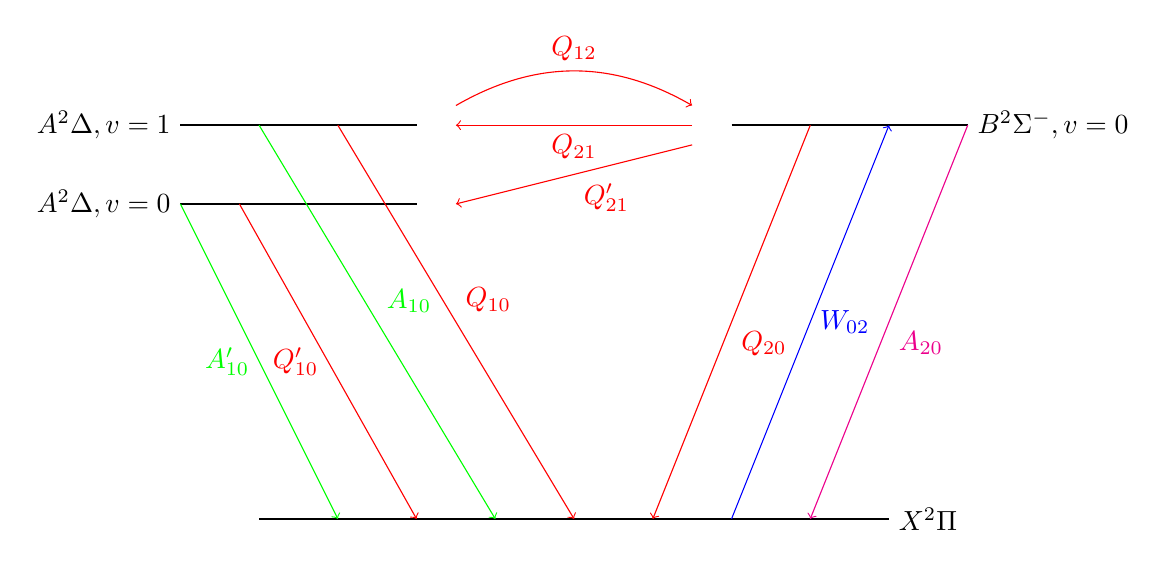
\begin{tikzpicture}

% Ground state
\draw [thick] ( 1, 0 ) -- ++( 8, 0 );
\node at ( 9, 0 ) [right] {\(X^2\Pi\)};

% First electronic states
\draw [thick] ( 0, 4 ) -- ++( 3, 0 );
\node at ( 0, 4 ) [left] {\(A^2\Delta, v = 0\)};
\draw [thick] ( 0, 5 ) -- ++( 3, 0 );
\node at ( 0, 5 ) [left] {\(A^2\Delta, v = 1\)};

% Second electronic state
\draw [thick] ( 7, 5 ) -- ++( 3, 0 );
\node at ( 10, 5 ) [right] {\(B^2\Sigma^-, v = 0\)};

% Transitions
\path [->, blue] ( 7, 0 ) edge node [right] {\(W_{02}\)} ++( 2, 5 );
\path [->, red] ( 8, 5 ) edge node [auto] {\(Q_{20}\)} ++( -2, -5 );
\path [->, magenta] ( 10, 5 ) edge node [auto] {\(A_{20}\)} ++( -2, -5 );

\path [->, red] ( 6.5, 5 ) edge node [auto] {\(Q_{21}\)} ++( -3, 0 );
\path [->, red] ( 6.5, 4.75 ) edge node [auto] {\(Q'_{21}\)} ++( -3, -0.75 );
\path [->, red] ( 3.5, 5.25 ) edge [bend left] node [above] {\(Q_{12}\)} ++( 3, 0 );

\path [->, red] ( 2, 5 ) edge node [auto] {\(Q_{10}\)} ++( 3, -5 );
\path [->, green] ( 1, 5 ) edge node [auto] {\(A_{10}\)} ++( 3, -5 );

\path [->, red] ( 0.75, 4 ) edge node [left] {\(Q'_{10}\)} ++( 2.25, -4 );
\path [->, green] ( 0, 4 ) edge node [left] {\(A'_{10}\)} ++( 2, -4 );

\end{tikzpicture}

\caption[Transitions in the improved CH fluorescence model]{A simplified model of the transitions between the energy levels in a CH system. Excitation (\textcolor{blue}{blue}) of ground state CH molecules to the upper electronic state is followed by several collisional energy transfer processes (\textcolor{red}{red}). A small portion of these molecules spontaneously emit a photon (\textcolor{green}{green}) and return to ground state. The spontaneous emission corresponding to resonant PLIF (\textcolor{magenta}{magenta}) is not collected.}

\label{fig:simplifiedEnergyLevels}

\end{figure}



The rates of the various transition processes are indicated in Figure \ref{fig:simplifiedEnergyLevels}.
\(W_{02}\) is the pumping process that populates the \(B\)(0) state.
\(Q_{ij}\) are collisional energy transfer processes that transfer CH molecules from the \(i\) level to the \(j\) level.
The subscripts 0, 1 and 2 represent the electronic energy levels \(X\), \(A\) and \(B\).
Processes involving the \(A\)(0) state are differentiated from those involving the \(A\)(1) state by a prime (\('\)).
Finally, \(A_{ij}\) represents the spontaneous emission coefficients between the \(i\) and \(j\) levels.

Applying Equation \ref{eqn:fluorescencePhotons} to this case, we can write an expression for the LIF signal intensity as follows,

\begin{equation}
  \Phi = ( n_1 A_{10} + n'_1 A'_{10} )V
  \label{eqn:signalIntensity}
\end{equation}

Our task is to solve for the values of \(n_1\) and \(n'_1\) in terms of \(n_0\).
To do this we need to write rate equations describing the variation of the populations of the three upper states with time.

\begin{align}
  \frac{dn_1}{dt} &= -( A_{10} + Q_{10} + Q_{12} )n_1 + Q_{21} n_2
  \label{eqn:rates1}\\
  \frac{dn'_1}{dt} &= -( A'_{10} + Q'_{10} )n'_1 + Q'_{21} n_2
  \label{eqn:rates2}\\
  \frac{dn_2}{dt} &= W_{02} n_0 + Q_{12} n_1 - ( A_{20} + Q_{20} + Q_{21} + Q'_{21} )n_2
  \label{eqn:rates3}
\end{align}

Under the assumption that the laser excitation time scale is much longer that the collisional time scales, we can set the LHS of Equations \ref{eqn:rates1}--\ref{eqn:rates3} to zero.
This results in a closed set of linear equations, which can be expressed in matrix form as follows.

\begin{equation}
  \left[
    \begin{matrix}
      A_{10} + Q_{10} + Q_{12} & 0 & -Q_{21}\\
      0 & A'_{10} + Q'_{10} & -Q'_{21}\\
      -Q_{12} & 0 & A_{20} + Q_{20} + Q_{21} + Q'_{21}
    \end{matrix}
  \right]\left[
    \begin{matrix}
      n_1\\
      n'_1\\
      n_2
    \end{matrix}
  \right] = \left[
    \begin{matrix}
      0\\
      0\\
      W_{02}n_0
    \end{matrix}
  \right]
  \label{eqn:closedForm}
\end{equation}

From Equation \ref{eqn:closedForm}, we only need the solutions to \(n_1\) and \(n'_1\).
These solutions are presented in Equations \ref{eqn:solution1}--\ref{eqn:solution2}.

\begin{align}
  n_1 &= n_0W_{02}Y
  \label{eqn:solution1}\\
  n'_1 &= n_0W_{02}Y'
  \label{eqn:solution2}
\end{align}.

The expressions for the respective flourescence yields, \(Y\) and \(Y'\) are as follows,

\begin{align}
  Y &= \frac{ Q_{21} }{ ( A_{10} + Q_{10} + Q_{12} )( A_{20} + Q_{20} + Q_{21} + Q'_{21} ) - Q_{12}Q_{21} }
  \label{eqn:flourescenceYield1-unsimplified}\\
  Y' &= \frac{ ( A_{10} + Q_{10} + Q_{12} )Q'_{21} }{ ( A'_{10} + Q'_{10} ) ( ( A_{10} + Q_{10} + Q_{12} )( A_{20} + Q_{20} + Q_{21} + Q'_{21} ) - Q_{12}Q_{21} ) }
  \label{eqn:fluorescenceYield2-unsimplified}
\end{align}

\subsubsection{Solution}
\label{subsubsec:improved-model-solution}

Substituting the expressions from Equations \ref{eqn:solution1}--\ref{eqn:solution2} into Equation \ref{eqn:signalIntensity},

\begin{equation}
  \Phi = n_0VW_{02}(Y + Y')
  \label{eqn:improvedModel-weak}
\end{equation}

Note the similarity in the form of Equation \ref{eqn:improvedModel-weak} to Equation \ref{eqn:twoLevelModel-weak}.
Both expressions are composed of two parts---a pumping rate and a fluorescence yield.
Expanding the pumping rate \(W_{02}\) in a manner identical to Equation \ref{eqn:pumpingRate} and using the absorption integral in Equation \ref{eqn:absorptionIntegral}, we can rewrite Equation \ref{eqn:improvedModel-weak} in a form mirroring Equation \ref{eqn:twoLevelModel}

\begin{equation}
  \Phi = \frac{P}{c} \int_x n_{CH} (Y + Y') \sum_j f_j B_j \int_\nu \psi(\nu) \phi_j(\nu) d\nu dx
  \label{eqn:improvedModel}
\end{equation}

The expressions for the fluorescence yields, \(Y\) and \(Y'\), still have many variables that have not been tabulated conveniently in literature.
As a result, further simplifications will need to be made on the basis of reported experimental observations.
These simplifications are outside the scope of this chapter and will be introduced in Chapter \ref{ch:chplif} along with the results of applying this model to various reactant mixtures.


\chapter{Experimental Methods and Considerations}

% It might be interesting to break up the chapter like this:
% 1. Experimental Facilities
%   a. LSB Test Rig A
%   b. LSB Test Rig B
%   c. Bunsen flame?
% 2. Diagnostic Techniques
%   a. LDV
%   b. CH* chemiluminescence
%   c. CH PLIF

The current chapter details the facilities and apparatus used to study the flame characteristics in a Low Swirl Burner.
The selection and implementation of diagnostic techniques used in this study are explained, as are data analysis methods used to process the acquired data.

\section{LSB configuration}

Two LSB configurations, A and B are tested for this study.
Each LSB configuration is built around a swirler with an outer diameter, \(d_s\) of 38 mm (1.5 in).
Other key dimensions of the swirlers tested for this work are presented in Table \ref{tab:swirlerdimensions}.

\begin{table}

\caption[Swirler Dimensions]{The dimensions of the swirlers used and the respective perforated plates are presented. Each swirler is referred to by its vane angle (as in ``\(S_{37^\circ}\)'').}

\begin{center}
\begin{tabular}{lcc}
  Geometric parameter & \multicolumn{2}{c}{Swirler} \tabularnewline
  & \(S_{37^\circ}\) & \(S_{45^\circ}\) \tabularnewline
  \hline \hline
  \textbf{Swirler data} & & \tabularnewline
  Outer diameter, \(d_s\), mm & 38 & 38 \tabularnewline
  Diameter ratio, \(\frac{d_i}{d_s}\) & 0.66 & 0.66 \tabularnewline
  Vane angle, \(\alpha\) & 37\(^\circ\) & 45\(^\circ\) \tabularnewline
  Theoretical Swirl Number, \(S\) & 0.48 & 0.64 \tabularnewline
  & & \tabularnewline
  \textbf{Perforated plate data} & & \tabularnewline
  Open area, mm\(^2\) & 155.97 & 156.98 \tabularnewline
  Blockage, \% & 71.54 & 71.36 \tabularnewline
  Plate thickness, mm & 1.27 & 1.27 \tabularnewline
  Hole pattern & 1 - 8 - 16 & 1 - 8 - 16 \tabularnewline
  Hole location (dia), mm & 0 - 10.2 - 19.1 & 0 - 10.2 - 19.1 \tabularnewline
  Hole diameter, mm & 2.79 - 2.79 - 2.84 & 2.82 - 2.82 - 2.83 \tabularnewline
\end{tabular}
\end{center}

\label{tab:swirlerdimensions}

\end{table}

Initial testing aimed at velocity field mapping and flame imaging is conducted on Configuration A, while Configuration B is used for a later series of tests aimed at visualizing the flame structure.
The design of these two configurations is discussed in further detail in what follows.

\subsection{Configuration A}

In this configuration, the reactants reach the swirler through a converging nozzle that decreases linearly in diameter from from the inlet diameter of 102 mm (4 in) to the outer diameter of the swirler, 38 mm (1.5 in).
The swirler leads to a constant area nozzle, and is located one diameter upstream of an abrupt area change.
At the area change, the reactants expand from the 38 mm (1.5 in) diameter nozzle into a 115 mm (4.5 in) diameter combustion zone.
The expansion ratio is chosen so as to avoid confinement effects on the centerline flame flow field.\cite{1998-yegian}

The main combustion zone begins at the dump plane and is enclosed by a GE 214 quartz tube.
The quartz tube is 300 mm (12 in) long and 115 mm (4.5 in) in diameter.
The thickness of the quartz tube is 2.5 mm (0.1 in).
Configuration A is illustrated in Figure FIXME.

\subsection{Configuration B}

In this configuration, the reactants approach the swirler through a smoothly contoured nozzle with a high contraction ratio designed to inhibit the formation of thick boundary layers.
The swirler again leads to a constant area nozzle which is FIXME diameters in length.
Following this, the reactants enter the combustion zone.

Unlike in Configuration A, there is no dump plane or quartz tube to provide confinement to the combustion zone.
Further, in this configuration, the annular flow is separately controlled from the central flow, which allows one to control the mass flow split directly, if needed.
Finally, this configuration allows for adjusting the level of turbulence present in the inlet flow by use of a turbulence generator located upstream.

The details of Configuration B are shown in Figure FIXME.

\section{High Pressure Test Rig}

Each of the two configurations is housed in a separate high pressure testing rig with optical access to study the flame.
These rigs consist of an air and fuel supply system, a pressure vessel with adequate optical access and an exhaust system.
The details of each rig are discussed in the following sub-sections.

\subsection{Test Rig A}

Preliminary experiments involving velocity field mapping and flame imaging are conducted in Test Rig A, shown in Figure FIXME.
Preheated air at about 500 K is drawn from external tanks and metered through an orifice flow meter.
The air enters the inlet nozzle of the LSB through a 1.8 m (6 ft) long, 102 mm (4 in) diameter straight pipe section.
Fuel (natural gas) is metered using another orifice flow meter and injected at the head of the straight pipe section.
The straight pipe section allows for the flow to be fully developed, and fully premixed before the reactants enter the burner.
The combustor pressure and temperature are measured at the head of the inlet nozzle by a pressure transducer and a thermocouple respectively.
In addition, the upstream pressure and the pressure differential are measured at the air and fuel orifice flow meters.
For the preheated air stream, the upstream temperature is also measured.
The measurements are used to calculate the four primary flow parameters (combustor pressure, preheat temperature, reference velocity and equivalence ratio) for the LSB in real time.
All measurements are monitored and recorded during the course of the experiment by a LabView VI.

The pressure vessel enclosing the combustor is designed to withstand pressures of up to 30 atm and is insulated from the combustor by a ceramic liner.
Cooling for the pressure vessel and the quartz tube is provided by a flow of cold air introduced at the head of the pressure vessel.
Optical access to the combustor is provided through four 150 mm (6 in) \(\times\) 75 mm (3 in) quartz windows located \(90^\circ\) apart azimuthally.
The view ports allow the combustor to be imaged from the dump plane to an axial distance of 150 mm (6 in) downstream.

The exhaust from the combustor is cooled by circulating cold water through a water jacket enclosing the exhaust pipe section.
The length of the exhaust pipe section is about FIXME.
The exhaust pipe section terminates in an orifice plug to provide the back pressure to the combustion chamber.
Different diameter orifices are used for each reference velocity condition to be tested.
The exiting products are finally released to the building exhaust system.

\subsection{Test Rig B}

FIXME

\section{Diagnostics}

\subsection{Laser Doppler Velocimetry}

The velocity field of the LSB is mapped using a TSI 3-component LDV system.
Three wavelengths (514 nm, 488 nm and 476 nm) are separated from the output of a 5 W Argon ion laser by an FBL-3 multicolor beam generator.
The individual beams are split into two coherent beams which are then focused to intersect and produce interference fringes within an ellipsoidal measurement volume with dimensions of the order of 100 \(\mu\)m.
For this purpose, two transceiver probes are mounted \(90^\circ\) apart about the axis of the LSB.
One transceiver probe focuses the 514 nm and 488 nm beams in planes perpendicular to each other, while the second probe focuses the 476 nm beams orthogonal to the other two beams.
Particles in the flow field crossing the interference fringes scatter the laser light elastically and produce a sinusoidal signal whose frequency is proportional to the velocity of the particle.
The transceiver probes collect this scattered light and each wavelength is detected separately by a PDM-1000-3 three-channel photodetector module.
The output from the photodetector is processed by an FSA-3500-3 signal processor.
The resulting three components of the particle/flow velocity are recorded by the FlowSizer software.

Since the airflow is very sparsely populated by particles, the flow needs to be artificially seeded to facilitate LDV measurements in a reasonable amount of time.
The seeding particles to be used and their mean diameter are decided by the characteristics of the flow to be imaged.\cite{1997-melling}
Since the LSB flow field is a reacting one, the particles need to have high melting points.
Further, the particles need to be small enough to follow the flow closely and large enough or reflective enough to scatter light efficiently in the measurement volume.
Based on these requirements, commercially available alumina particles with a mean particle diameter of 5 \(\mu\)m were chosen for this study.
In order to uniformly seed the flow, a novel seeding generator was designed as described in Appendix \ref{app:seeder}.
The seeding particles were introduced slightly upstream of the 1.8 m (6 ft) long straight pipe section in Test Rig A.

LDV data is only acquired at atmospheric pressure conditions.
At high pressure conditions, the reacting LSB flow field produces sharp refractive index gradients that rapidly shift in the turbulent flow field.
This causes strong beam steering effects making it very difficult for the laser beams to reliably intersect within such a small measurement volume.
The long distance traveled by the beams in the test rig further exacerbated this problem, making LDV data nearly impossible to acquire at such conditions.

\subsection{CH* chemiluminescence}

The LSB flame is imaged using one of two 16-bit intensified CCD cameras --- PI Acton 1024\(\times\)256 or 512\(\times\)512 pixels --- with a 28 mm f/2.8 camera lens.
CH* chemiluminescence is filtered using a bandpass filter centered on 430 nm with a FWHM of 10 nm.
At each operating condition, 100 instantaneous images are acquired with an exposure of 1 ms.
An additional 100 instantaneous images are acquired with no flame and averaged to yield the background for correcting the flame images.

CH* chemiluminescence has several advantages over flame chemiluminescence from other radicals such as OH*, \ce{C2}*, etc.
First, the CH* emission occurs around 430 nm and is not affected by blackbody radiation from the walls of the combustor.
\ce{C2}*, on the other hand, emits around 514 nm and is significantly affected by this issue.
Second, the intensity of the chemiluminescence from CH* is known to scale well with heat release in the combustor\cite{2006-hardalupas}, unlike \ce{C2}*.
Third, the emitted light can be gathered with high quantum efficiency by the intensified CCD cameras used for this study.
The quantum efficiency of the 18 mm Gen III HB filmless intensifier used by the 512\(\times\)512 camera is about 45\% at 430 nm, compared to about 10\% at 310 nm, where OH* chemiluminescence peaks.

\subsubsection{Image Processing}

The flame chemiluminescence images acquired are background-corrected and averaged.
The resulting mean is the line-of-sight integrated, time-averaged image of the flame.
Strictly speaking, this is not the same as a real average obtained from a long exposure image.
The instantaneous images are obtained through a periodic sampling process and hence, are prone to statistical errors and aliasing.
However, the behaviour of the flame can be assumed to be sufficiently random, and the mean obtained is adequately representative of the true average.
Figure FIXME shows a typical mean CH* chemiluminescence image prepared in this manner.

% what can you do with the average image?
Even when background-corrected, the walls of the combustor are not at zero intensity in the average chemiluminescence image.
This is particularly visible near the dump plane where there is no flame present and yet the walls are reasonably visible.
This is caused mostly by scattered chemiluminescence from the flame itself, and to a lesser degree, by blackbody radiation from the heated walls.
The averaged chemiluminescence image allows us to measure the flame standoff distance by following the intensity profile along the centerline of the combustor.
The intensity profile rises sharply when passing the flame standoff location.
Thus, the flame standoff location can be ascertained by finding the inflection point in the intensity profile.

The profile of the average chemiluminescence intensity along the centerline of the sample case from Figure FIXME is shown in Figure FIXME, showing the flame standoff distance.
The distance from the dump plane, measured in number of pixels on the image and scaled by the appropriate magnification factor yields the flame standoff distance, \(X_f\).
The determination of the flame standoff location by this method provides a suitable and deterministic means to locating the leading edge of the flame front.
\nomenclature{\(X_f\)}{Flame standoff distance}

The average image can be processed further to yield more spatially resolved information about the flame brush.
Under the reasonable assumption that the average LSB flame is axially symmetric about the centerline of the combustor, a tomographic deconvolution technique called the Abel deconvolution\cite{1992-dasch} can be used to convert the line-of-sight integrated image to a radial map of chemiluminescence intensity.
In effect, this shows the shape and structure of the average flame brush.
The Abel deconvolution of the sample data from Figure FIXME is shown in Figure FIXME.

The Abel-deconvoluted image provides an relatively easy means to determining the angle of the flame brush.
A straight line joining two points located at the center of the flame brush intersects the axis of the combustor at this angle.
The angle of the flame is denoted by \(\theta_f\).

Using the Abel deconvolution to study the flame brush suffers from two main drawbacks.
First, the system of equations describing the Abel deconvolution is only valid as long as the entirety of the flame is visible.
This is only satisfied in the initial region of the LSB where the diameter of the flame brush is smaller than the height of the optical viewport.
At further downstream locations, the flame is not imaged in its entirety.
This causes the spurious bright regions near the top of the window in Figure FIXME.
The second limitation of the Abel deconvolution technique stems from the high incidence of errors along the centerline (where \(r \to 0\)).
Due to this, any study of the flame brush thickness at the flame stabilization point --- a metric of considerable importance --- is all but impossible using this tomographic technique.

\subsection{CH Planar Laser Induced Fluorescence}

The CH PLIF setup uses the frequency-doubled output of a Light Age PAL 101 alexandrite laser tuned to \(\lambda \approx 387.2\) nm to pump the R-bandhead of the CH \(B^2\Sigma^- \leftarrow X^2\Pi\) (0,0) system.
This populates the \(A^2\Delta\) state through fast electronic energy transfer from the \(B^2\Sigma^-\) state.
The resulting broadband fluorescence observed between \(\lambda\) = 420--440 nm is due to the \(A^2\Delta \rightarrow X^2\Pi\) (1,1), \(A^2\Delta \rightarrow X^2\Pi\) (0,0) and \(B^2\Sigma^- \rightarrow X^2\Pi\) (0,1) bands.
The CH PLIF signal is collected using an intensified PI Acton 512\(\times\)512 camera equipped with an 18 mm Gen III HB filmless intensifier with a quantum efficiency of about 45\% in the 420--440 nm range.
Elastic scattering from the laser beam is attenuated by a 3 mm thick GG 420 Schott Glass filter.

\subsubsection{Laser Wavelength Calibration}

The output of the PAL 101 alexandrite laser is controlled using a micrometer-coupled frequency selection element in the laser cavity.
The manufacturer-supplied calibration for the micrometer was found to be incorrect.
This required the recalibration of the laser in order to know the correspondence of the micrometer settings to the output wavelength.

The laser output was calibrated using an Ocean Optics HR 2000 spectrometer.
The spectrometer is calibrated using 50 wavelengths in the 400--850 nm range from output of an Neon discharge lamp source.
The spectrometer is also intensity corrected over this range using a black body source.
The estimated error in the resolution of the device is about 0.1 nm.

The laser micrometer was traversed from 0.600 in to 0.626 in and back in steps of 0.001 in.
Spectra were recorded for these settings integrated over 512 ms and averaged over 10 acquisitions.
The calibration was performed using the fundamental wavelength of the laser.

Each acquired spectrum was modeled as a Gaussian profile and the location of the center wavelength was noted.
The variation of the wavelength is verified to be linear against the micrometer setting (as specified by the manufacturer) and the correct calibration equation is obtained by doing a linear curve fit of the data.
The results are shown in Figure FIXME.

\subsubsection{Excitation scan}

% This section needs a rewrite.

For this analysis, a premixed, stoichiometric, laminar methane-air flame is imaged by the CH PLIF imaging system.
The laminar flame is stabilized on a Bunsen burner with an inner diameter of 10.16 mm (0.4 in).
The alexandrite laser is operated at 10 Hz, with a power of 16 mJ/pulse.
The optics form the second harmonic beam into a sheet about 25 mm tall with a thickness on the order of 100 \(\mu\)m passing through the center of the flame.
The edges of the sheet are blocked by razor blades.
The excitation scan is performed by tuning the output of the laser from \(\lambda\) = 387.077 nm to 387.260 nm.

The induced fluorescence is imaged perpendicularly by the intensified camera using an 85 mm f/1.8 Nikon AF Nikkor lens and the intensifier is gated over 300 ns.
100 instantaneous images are acquired for each case.
The resolution of the imaging system is approximately 62 \(\mu\)m per pixel.

Figure FIXME shows a sample CH PLIF image from this dataset.
The images are background-corrected and the signal statistics are measured at the midpoint of the flame.
The CH PLIF signal mean is thresholded and scaled to match the normalized value of the simulation profile at the peak.
The results agree extremely well with the simulated profile of the R-bandhead.
This validates our calibration of the laser wavelength and our calculation of the laser linewidth.
Finally, this shows that the optimal excitation wavelength is about 387.2 nm.


\chapter{CH PLIF Signal Modeling and Validation}
\label{ch:chplif}

% This chapter covers the modeling of the CH PLIF signal and contains the following sections:

% 0. Preliminary experiments
%   0.1 Excitation scan
%   0.2 Linearity test
% 1. Signal modeling
%     1.1 Constants, assumptions, simplifications
%     1.2 Comparison of models (GRI, USCv2, Syngas, C1-C3, San Diego, etc.) / CH₄+air results
% 2. Results
%   Unstrained, laminar flames
%     2.1 Methane + air flames
%         2.1.1 subsection comparison with experiments
%     2.2 C1-C3 alkanes flames
%     2.3 Syngas mixtures
%     2.4 Syngas + C1-C3 alkanes
%   Strained laminar flames
%     2.5 Strain effects

% Questions to be answered (from proposal):

% 1. Detailing the development of a CH PLIF system (covered in Chapter 2,3 and here)
% 2. Demonstration on an atmospheric pressure laminar flame
% 3. Validate with quenching models
% 4. Model signal for strained flames
% 5. Model signal for fuel mixtures

% TODO:Write a short introduction to the chapter to start it off

\section{CH PLIF Preliminary Experiments}
\label{sec:chplif-preliminary-experiments}

The CH PLIF imaging system was evaluated for use in imaging hydrocarbon flames by performing two preliminary experiments.
First, an excitation scan was performed to locate the optimal wavelength to excite the CH radicals in a typical hydrocarbon flame.
The variation in this optimal wavelength with temperature and pressure was calculated and found to be within acceptable bounds.
Second, a test of the linearity of the LIF signal with respect to the incident laser intensity was performed.
The setup and results of these experiments are described in the following subsections.

\subsection{Excitation Scan}
\label{subsec:prelim-excitation-scan}

An excitation scan is performed by tuning the output of the alexandrite laser from \(\lambda\) = 387.077 nm to 387.260 nm.
This serves two purposes.
First, it locates the optimal wavelength to excite the CH radicals that results in the highest fluorescence yield.
Second, the variation of the signal intensity can be compared with simulated profiles from LIFBASE or other spectroscopic calculations and our estimation of the laser linewidth can be validated.
The laser linewidth is an integral parameter and appears in the absorption integral used by the models developed in Chapter \ref{ch:background}.

A schematic of the excitation scan experiment is shown in Figure FIXME.
The intensified PI Acton 512\(\times\)512 camera described in Section \ref{subsec:experimental-ch-chemiluminescence} is used to image a premixed, laminar methane-air flame operating at close to stoichiometric conditions.
The laminar flame is stabilized on the Bunsen burner described in Section \ref{subsubsec:plif-laminar-flame-setup}.
The alexandrite laser is operated at a power of 16 mJ/pulse in the second harmonic.
The sheet forming optics consist of a +50 mm cylindrical lens and a +250 mm spherical lens placed 300 mm apart.
The optics form the beam into a collimated sheet about 25 mm (1 in) tall, focused to a thickness on the order of 100 \(\mu\)m at the flame location.
The sheet passes through the center of the flame and the edges of the sheet are blocked by razor blades to prevent reflections from the burner from saturating the camera.

The induced fluorescence in the flame sheet is imaged perpendicularly by the intensified camera using an 85 mm f/1.8 Nikon AF Nikkor lens.
This gives a magnification of approximately 62 \(\mu\)m/pixel.
The camera is triggered by the flash lamp sync signal from the laser system and the intensifier is gated over 300 ns, encompassing the 70 ns laser pulse.
The long gate width gives the intensifier enough time to prepare to receive the fluorescence, preventing signal loss due to irising.
The gate width is still short enough that minimal flame chemiluminescence or ambient lighting is recorded in the images.
100 instantaneous images are acquired for each excitation wavelength to acquire a good estimate of the mean fluorescence signal, \(\mu_{sig}\).

Figure FIXME shows a sample CH PLIF image from this dataset.
The images are background-corrected by subtracting the laser scattering (recorded without the flame).
The fluorescence signal is calculated from these images using three alternate approaches.

In Method I, two ``windows'' are identified that include the straight sections of the laminar flame.
The average fluorescence signal in each frame is calculated by taking the average of all the emitting pixels in the two windows.
A pixel is designated as an emitting pixel if its intensity exceeds the standard deviation of a typical background pixel by at least a factor of five.
The average of this value over all the frames is designated as the mean fluorescence signal, \(\mu_{sig}\).
In Method II, the intensity of the pixels is integrated over a straight line connecting the inner and outer edges of the flame.
The straight line is chosen along the beam so that the beam intensity does not vary along the integration path.
The integration is performed on the left and right arms of the flame, giving two readings per frame.
The mean of these values over all the frames is recorded as the mean fluorescence signal, \(\mu_{sig}\).
In Method III, the midpoints of the straight lines from Method II are located and the average of their intensities, over all the frames is recorded as the mean fluorescence signal, \(\mu_{sig}\).
The regions of interest for each of these methods is highlighted in Figure FIXME.

The result of this investigation is shown in Figure FIXME.
The calculated mean fluorescence signals from the three methods are plotted against a LIFBASE simulation of the absorption spectrum of the CH \(B-X\) transition.
The profiles are appropriately scaled to match the LIFBASE simulation at the maximum value and at the minimum value.
The LIFBASE simulation is performed for a thermalized system at 1800 K, at atmospheric pressure.
Further, the instrument linewidth is specified to be the same as our estimate of the laser linewidth (1.06 \AA).

The profiles of the calculated and scaled mean fluorescence signals are observed to agree extremely well with the LIFBASE simulation result.
The discrepancies between the three methods is minimal.

The results indicate that the optimal excitation wavelength, corresponding to the highest mean fluorescence signal, is about 387.2 nm.
For the rest of the experiments performed in this work, the laser is operated at this wavelength.
The results also help verify that the calibration of the micrometer is accurate and the wavelengths are precisely adjustable.
Finally, the results validate that our estimated laser linewith, 1.06 \AA, is accurate.
This value can now be used in subsequent calculations of the LIF signal levels.

\subsection{Linearity Test}
\label{subsec:prelim-linearity-test}

As explained in Chapter \ref{ch:background}, the variation of the fluorescence signal with the excitation laser intensity exhibits a saturation curve.
For reasons mentioned in that discussion, we prefer to operate in the weak excitation limit.
Further, the models developed in Chapter \ref{ch:background} for calculating the signal are intended to be used in the linear regime.
Hence, an experiment is performed to verify the linearity of the system response at the intensities at which the flames are imaged for this work.
The schematic of the setup is shown in Figure FIXME.
The laser is tuned to the optimal wavelength as determined in Section \ref{subsec:prelim-excitation-scan}, and operated at 10 Hz.
The frequency-doubled beam is directed at a steady, laminar, methane-air Bunsen flame operating at a slightly rich stoichiometry.
The edges of the beam are clipped by an aperture to produce a sharp edge and to avoid unnecessary reflections from the burner.
No optics are used to refract the beam in any way.

The flame is imaged by the PI Acton 512\(\times\)512 intensified camera equipped with a 50 mm, f/1.8 AF Nikkor lens.
Elastic scattering is attenuated by a 3 mm thick GG 420 Schott glass filter.
The magnification achieved by this set up is about 44 \(\mu\)m/pixel.
The LIF signal from the flame is recorded in 300 ns gates and accumulated 150 times before being read out.
For each case, a corresponding laser scattering image is also recorded for estimating the background.
The flame chemiluminescence and ambient background are also recorded for the same purpose.

For this experiment, varying the intensity of the laser beam by changing the flash lamp voltage or even the Q-switch timing is not preferred as either would alter the pulse width of the beam.
Instead, quartz disks and blocks of varying thickness are introduced into the beam to produce an intensity loss, while preserving all other characteristics of the beam.
The quartz elements decrease the intensity of the laser beam through reflection, scattering and absorption.
The stray reflections and scattering from the quartz elements are contained by enclosing the elements in a box and preventing these from being recorded by the camera.
In this manner, the laser power is varied from 10 mJ/pulse to 0.5 mJ/pulse and back.

The acquired images are background-corrected and the intensity is conditionally averaged over pixels with a non-zero intensity in the region where the fluorescence occurs.
The average fluorescence intensity values thus obtained are plotted against the corresponding laser intensity and shown in Figure FIXME.
A sample image highlighting the region of interest is also shown alongside.

The LIF signal is observed to increase monotonically with increasing laser intensity.
At the lower intensities, the variation is very nearly linear, with marginal scatter and only one significant outlier.
At intensities above 1 J/cm\(^2\) however, there is significant scatter in the data and the linear trend obtained from the low intensity cases cannot be reliably extended over this region.

The results indicate that as long as the intensity of the laser sheet is kept below 1 J/cm\(^2\), the assumption of operating in the linear regime is valid.

\section{Fluorescence Signal Modeling}
\label{sec:chplif-fluorescence-signal-modeling}

Chapter \ref{ch:background} presented analysis of LIF signal calculation as a function of thermodynamic conditions and the local composition in a flame.
Expressions derived using a basic model (Equation \ref{eqn:twoLevelModel}) and a more complex model (Equation \ref{eqn:improvedModel}) were presented.
The expressions rely on knowledge of several physical values and specific spectroscopic constants pertaining to the CH system.

\begin{table}
  \caption[CH emission coefficients]{The coefficients of spontaneous emission for transitions in the CH system are provided.}
  \begin{center}
    \begin{tabular}{lcr}
      Transition & Symbol & A \tabularnewline
      & & \(\times 10^6\) s\(^{-1}\) \tabularnewline
      \hline\hline
      & & \tabularnewline
      \(B^2\Sigma^-\rightarrow X^2\Pi(0,0)\) & \(A_{20}\) & 2.963 \tabularnewline
      \(A^2\Delta\rightarrow X^2\Pi(1,1)\) & \(A_{10}\) & 1.676 \tabularnewline
      \(A^2\Delta\rightarrow X^2\Pi(0,0)\) & \(A'_{10}\) & 1.832 \tabularnewline
      \hline
    \end{tabular}
  \end{center}
  \label{tab:emissionCoefficients}
\end{table}



The basic model requires us to know the Einstein coefficient for spontaneous emission from the ``upper'' state to the ``lower'' state.
For this, we assume that the ``upper'' state has the same properties as the \(A^2\Delta\), \(v = 0\) state.
The improved model, needs the emission coefficients for the \(B^2\Sigma^-\), \(v = 0\) and \(A^2\Delta\), \(v =\) 0, 1 states.
These are tabulated from sources in literature\cite{1985-garland-a,1996-luque-b} FIXME in Table \ref{tab:emissionCoefficients}.

\begin{table}
  \caption[CH quenching cross-sections]{The functional form of the quenching cross-sections of various species with CH are provided.}
  \begin{center}
    \begin{tabular}{lr}
      Species & \(\sigma\), \AA\(^2\) \tabularnewline
      \hline\hline
      \ce{H2} & \(6.1 \exp{ \left(-686 / T \right)}\) \tabularnewline
      \ce{H} & \(221 T^{-0.5} \exp{ \left( -686 / T \right)}\) \tabularnewline
      \ce{O2} & \(8.61 \times 10^{-6} T^{1.64} \exp{ \left( 867 / T \right)}\) \tabularnewline
      \ce{OH} & \(221 T^{-0.5} \exp{ \left( -686 / T \right)}\) \tabularnewline
      \ce{H2O} & 9.6 \tabularnewline
      \ce{CH4} & \(52.8 T^{-0.5} \exp{ \left( -84 / T \right)}\) \tabularnewline
      \ce{CO} & 8.31 \tabularnewline
      \ce{CO2} & \(8.67 \times 10^{-13} T^{3.8} \exp{ \left( 854 / T \right)}\) \tabularnewline
      \ce{C2H6} & 13.4 \tabularnewline
      \ce{N2} & \(1.53 \times 10^{-4} T^{1.23} \exp{ \left( -522.1 / T \right)}\) \tabularnewline
      \ce{C3H8} & 22 \tabularnewline
      \hline
    \end{tabular}
  \end{center}
  \label{tab:quenchingCrossSections}
\end{table}



Next, to calculate the fluorescence yield for the basic model, we need to know the quenching cross-sections of major species found in the flames of interest.
These cross sections are curve-fitted from several experiments performed over varying ranges of temperature.
The functional forms of these cross-sections are presented in Table \ref{tab:quenchingCrossSections}.

The fluorescence yield expressions for the complex model require the rates of collisional transfer between several energy levels.
There have been efforts to measure and model these rates, but the energy level model used for these studies is more complicated and cannot be easily reconciled with our simplified model.
Hence, it would be preferable to make some simplifying assumptions so that the collisional rates can be reduced in terms of the quenching rate.

Previous work has reported that the rate of quenching does not appreciably vary over the vibrational manifold, but excited CH molecules in the \(B^2\Sigma^-\) electronic state are approximately 30\% more likely to be quenched than molecules in the \(A^2\Delta\) states.
This allows us to eliminate \(Q'_{10}\) and \(Q_{20}\) as follows.

\begin{gather}
  Q'_{10} = Q_{10} = Q
  \label{eqn:quenchingAssumption1}\\
  Q_{20} = 1.3Q
  \label{eqn:quenchingAssumption2}
\end{gather}

Our next assumption is based on work by Luque et al.\cite{2000-luque} FIXME who reported that the rate of transfer following the \(B^2\Sigma^-\rightarrow A^2\Delta\) (0,1) transition accounts for almost 24\% of the collisional removal of CH from the upper electronic state.
This allows us to formulate one more equation as shown below.

\begin{gather}
  \frac{ Q_{21} + Q'_{21} - Q_{12} }{ Q_{20} + Q_{21} + Q'_{21} - Q_{12} } = 0.24\\
  \therefore \frac{ R_{21} + R'_{21} - R_{12} }{ Q } = 0.4105
  \label{eqn:QEquation1}
\end{gather}

Next, using the reported results from the same authors\cite{2000-luque} FIXME, we know that the number of CH molecules following the \(B^2\Sigma^-\rightarrow A^2\Delta\) (0,1) transition is four times as much as the number following the \(B^2\Sigma^-\rightarrow A^2\Delta\) (0,0) transition.

\begin{equation}
  \frac{ Q_{21} - Q_{12} }{ Q'_{21} } = 4
  \label{eqn:QEquation2}
\end{equation}

Finally, Garland et al.\cite{1985-garland-b} FIXME reported that the rate of the forward transfer along the \(B^2\Sigma^-\rightarrow A^2\Delta\) (0,1) transition is about 60\% faster than the reverse process.

\begin{equation}
  \frac{Q_{21}}{Q_{12}} = 1.6
  \label{eqn:QEquation3}
\end{equation}

This gives us the third equation forming a closed, linear set of equations in terms of \(Q_{21}\), \(Q_{12}\) and \(Q'_{21}\) that can be written out in matrix form and solved.
Equation \ref{eqn:QSolution} presents the solution.

\begin{equation}
  \left[
    \begin{matrix}
      R_{21}\\
      R'_{21}\\
      R_{12}
    \end{matrix}
  \right] = \left[
   \begin{matrix}
      5.1966\\
      0.4872\\
      3.2479
    \end{matrix}
  \right] Q
  \label{eqn:QSolution}
\end{equation}

Substituting Equations \ref{eqn:quenchingAssumption1}, \ref{eqn:quenchingAssumption2} and \ref{eqn:QSolution} into Equations \ref{eqn:flourescenceYield1-unsimplified}--\ref{eqn:fluorescenceYield2-unsimplified} leads to simplified expressions for the two fluorescence yields.
More importantly, they are now functionally dependent on only the Einstein coefficients and the rate of collisional quenching.

\begin{align}
  Y_1 &= \frac{ 5.1966Q }{ ( A_{10} + 4.2479Q )( A_{20} + 6.9838Q ) - 16.8780Q }
  \label{eqn:fluorescenceYield1}\\
  Y'_1 &= \frac{ 0.4872Q( A_{10} + 4.2479Q ) }{ ( A'_{10} + Q ) \left( ( A_{10} + 4.2479Q )( A_{20} + 6.9838Q ) - 16.8780Q \right) }
  \label{eqn:fluorescenceYield2}
\end{align}

\begin{table}
  \caption[Absorption lines and coefficients for the \(B^2\Sigma^-\leftarrow X^2\Pi\) (0,0) R branch]{The line positions and the corresponding Einstein coefficients for stimulated absorption for transitions in the \(B^2\Sigma^-\leftarrow X^2\Pi\) (0,0) R branch are presented below.}
  \begin{center}
    \begin{tabular}{lcccccc}
      \(N''\) & \(J''_1\) & \(\nu_1\) & \(B\) & \(J''_2\) & \(\nu_2\) & \(B\) \tabularnewline
        & & cm\(^{-1}\) & \(\times10^{-9}\) m\(^2\)J\(^{-1}\)s\(^{-1}\) & & cm\(^{-1}\) & \(\times10^{-9}\) m\(^2\)J\(^{-1}\)s\(^{-1}\) \tabularnewline
      \hline\hline
      & & & & & & \tabularnewline
      1  & 0.5  & 25756.08 & 6.511 & 1.5  & 25774.03 & 5.823 \tabularnewline
      2  & 1.5  & 25776.42 & 7.225 & 2.5  & 25782.72 & 6.489 \tabularnewline
      3  & 2.5  & 25792.74 & 7.532 & 3.5  & 25797.06 & 7.174 \tabularnewline
      4  & 3.5  & 25805.42 & 7.671 & 4.5  & 25808.75 & 7.460 \tabularnewline
      5  & 4.5  & 25814.47 & 7.719 & 5.5  & 25817.20 & 7.581 \tabularnewline
      6  & 5.5  & 25819.80 & 7.708 & 6.5  & 25822.13 & 7.610 \tabularnewline
      7  & 6.5  & 25821.28 & 7.652 & 7.5  & 25823.32 & 7.581 \tabularnewline
      8  & 7.5  & 25818.72 & 7.561 & 8.5  & 25820.55 & 7.506 \tabularnewline
      9  & 8.5  & 25811.93 & 7.439 & 9.5  & 25813.59 & 7.396 \tabularnewline
      10 & 9.5  & 25800.64 & 7.288 & 10.5 & 25802.17 & 7.254 \tabularnewline
      11 & 10.5 & 25784.57 & 7.111 & 11.5 & 25785.98 & 7.083 \tabularnewline
      12 & 11.5 & 25763.38 & 6.907 & 12.5 & 25764.70 & 6.884 \tabularnewline
      13 & 12.5 & 25736.65 & 6.676 & 13.5 & 25737.88 & 6.657 \tabularnewline
      14 & 13.5 & 25703.90 & 6.418 & 14.5 & 25705.06 & 6.402 \tabularnewline
      15 & 14.5 & 25664.54 & 6.129 & 15.5 & 25665.64 & 6.116 \tabularnewline
      16 & 15.5 & 25617.87 & 5.815 & 16.5 & 25618.92 & 5.804 \tabularnewline
      17 & 16.5 & 25563.03 & 5.472 & 17.5 & 25564.03 & 5.463 \tabularnewline
      18 & 17.5 & 25499.00 & 5.101 & 18.5 & 25499.95 & 5.094 \tabularnewline
      19 & 18.5 & 25424.52 & 4.624 & 19.5 & 25425.42 & 4.618 \tabularnewline
      20 & 19.5 & 25338.08 & 4.161 & 20.5 & 25338.93 & 4.156 \tabularnewline
      21 & 20.5 & 25237.84 & 3.674 & 21.5 & 25238.64 & 3.670 \tabularnewline
      22 & 21.5 & 25121.60 & 3.183 & 22.5 & 25122.36 & 3.180 \tabularnewline
      \hline
    \end{tabular}
  \end{center}
  \label{tab:absorptionLines}
\end{table}



The calculation of the quenching rate also requires us to know the number density of the major species in the flame zone.
The profile of the local mole fractions of various species through a 1-D, freely propagating, laminar flame was obtained from CHEMKIN solutions using the Flame-Speed Calculator reactor model.
Results are presented in this chapter for laminar flames using a variety of reactant mixtures and inlet conditions.
Additional results for strained laminar methane-air flames are calculated using the Opposed flow flame reactor model.

The CHEMKIN results provide mole fractions, which can be used to solve for the number density of each species using the following equation.

\begin{equation}
  n_i = \frac{pN_AX_i}{RT}
  \label{eqn:numberDensity}
\end{equation}

In Equation \ref{eqn:numberDensity}, \(N_A\) is Avogadro's number, \(X_i\) is the mole fraction of species \(i\), \(R\) is the universal gas constant and \(p\), \(T\) are the local pressure and temperature in the flame.

Next, in order to calculate the absorption integral, we require the Einstein B-coefficients, along with the line positions of the transitions excited by the laser.
These are taken from FIXME and tabulated in Table \ref{tab:absorptionLines}.
Using these values, it is possible to calculate the optimal laser wavelength that results in the highest value of the absorption integral.
The optimal laser wavelength is not a constant value and depends on the temperature and pressure at which the CH molecules are present.
Using a typical value of 1800 K for the temperature in the flame zone, the variation of the optimal laser wavelength can be plotted against combustor pressure.
As the combustor pressure increases, the absorption lines in the CH \(B^2\Sigma^-\leftarrow X^2\Pi\) (0,0) R-bandhead are increasingly broadened by collisional broadening.
Absorption lines that are at slightly lower frequencies, but close to the bandhead can now begin to absorb the laser energy.
This causes the optimal laser wavelength to move slightly towards smaller wavenumbers.
Figure FIXME shows this variation.

During experiments, this shift contributes negligibly towards increasing the LIF signal and hence, the laser tuner can be left at the optimal location for atmospheric pressure cases.

\begin{table}
  \caption[Spectroscopic constants]{Spectroscopic constants for the CH \(X^2\Pi\) level are presented.}
  \begin{center}
    \begin{tabular}{lr}
      Constant & Value, cm\(^{-1}\) \tabularnewline
      \hline\hline
      \(\omega_e\) & 2860.7508 \tabularnewline
      \(\omega_ex_e\) & 64.4387 \tabularnewline
      \(\omega_ey_e\) & 0.36345 \tabularnewline
      \(\omega_ez_e\) & \(-1.5378 \times 10^{-2}\) \tabularnewline
      \(B_e\) & 14.459883 \tabularnewline
      \(\alpha_e\) & 0.536541 \tabularnewline
      \(D_e\) & \(1.47436 \times 10^{-3}\) \tabularnewline
      \(\beta_e\) & \(-2.530 \times 10^{-5}\) \tabularnewline
    \end{tabular}
  \end{center}
  \label{tab:spectroscopicConstants}
\end{table}


Returning back to Equations \ref{eqn:twoLevelModel} and \ref{eqn:improvedModel}, we need spectroscopic constants of the \(X^2\Pi\), \(v=0\) energy level in order to calculate the Boltzmann fractions, \(f_j\).
These constants have been determined by Zachwieja et al.\cite{1995-zachwieja} and are tabulated in Table \ref{tab:spectroscopicConstants}.


This formulation of the signal intensity implicitly makes the following assumptions.
\begin{enumerate}
\item The fluorescence emission is predicted at steady state.
\item The collection volume is optically thin and an emitted photon is not reabsorbed within the flame itself.
This is a reasonable assumption to make, since the flame thickness and the thickness of the laser sheet are both typically quite small.
\end{enumerate}

% Transplanted text. Needs to be integrated into Chapter 4

%  n_2 &= \frac{ ( A_{10} + Q_{10} + Q_{12} ) }{ ( A_{10} + Q_{10} + Q_{12} )( A_{20} + Q_{20} + Q_{21} + Q'_{21} ) - Q_{12}Q_{21} }W_{02}n_0

%The spontaneous emission coefficients, \(A_{10}\), \(A'_{10}\) and \(A_{20}\) are obtained from various published papers\cite{1985-garland-a,1996-luque-b,2005-richmond}.
%The values used for this analysis are presented in Table \ref{tab:emissionCoefficients}.


%Equations \ref{eqn:rates1}--\ref{eqn:rates3} describe the time variation of the number density of CH radicals in each excited state.

%At steady state, the rate of change of the number density is minimal.
%Under this assumption, the LHS of Equations \ref{eqn:rates1}--\ref{eqn:rates3} can be set to zero.
%This results in a closed set of linear equations in terms of the populations of the upper states.
%This set of equations is presented in Equation \ref{eqn:closedForm}.

%These expressions can be further simplified by noting various observations made in studies of the CH system.
%For instance, previous work\cite{1984-cool,1985-garland-b} has reported that the \(B\) state is slightly (about 1.3 times) more prone to quenching compared to the \(A\) state.
%We can thus make the following assumptions.


%Next, it has been reported\cite{2000-luque} that the electronic energy transfer rate from \(B\) to \(A\) state accounts for 0.24 times the total collisional removal from the \(B\) state.


%We further know\cite{1985-garland-b, 2000-luque} that the collisional transfer from the \(B(0)\) energy level populates the nearly degenerate \(A(1)\) level about four times faster than the \(A(0)\) level.


%Finally, it was observed\cite{1985-garland-b} that the rate of forward transfer from \(B(0)\) to \(A(1)\) is about 1.6 times the reverse process.



%Collating Equations \ref{eqn:REquation1}--\ref{eqn:REquation3}, we obtain a closed set of linear equations.
%This can be solved to eliminate \(R_{21}\), \(R_{12}\) and \(R'_{21}\) in terms of \(Q\) as shown in Equation \ref{eqn:RSolution}.

%\begin{equation}
%  \left[
%    \begin{matrix}
%      R_{21}\\
%      R'_{21}\\
%      R_{12}
%    \end{matrix}
%  \right] = \left[
%    \begin{matrix}
%      5.1966\\
%      0.4872\\
%      3.2479
%    \end{matrix}
%  \right] Q
%  \label{eqn:RSolution}
%\end{equation}

%Substituting Equations \ref{eqn:quenchingAssumption1}, \ref{eqn:quenchingAssumption2} and \ref{eqn:RSolution} into Equations \ref{eqn:solution1}--\ref{eqn:solution2} leads to simplified expressions for the populations of the upper electronic states purely as a function of the respective Einstein coefficients and the collisional quenching rate.
%These are presented in the following Equations \ref{eqn:simplifiedSolution1}--\ref{eqn:simplifiedSolution3}.

%\begin{align}
%  n_1 &= \frac{ 5.1966Q }{ ( A_{10} + 4.2479Q )( A_{20} + 6.9838Q ) - 16.8780Q } W_{02}n_0
%  \label{eqn:simplifiedSolution1}\\
%  n'_1 &= \frac{ 0.4872Q( A_{10} + 4.2479Q ) }{ ( A'_{10} + Q ) \left( ( A_{10} + 4.2479Q )( A_{20} + 6.9838Q ) - 16.8780Q \right) } W_{02}n_0
%  \label{eqn:simplifiedSolution2}\\
%  n_2 &= \frac{ ( A_{10} + 4.2479Q ) }{ ( A_{10} + 4.2479Q )( A_{20} + 6.9838Q ) - 16.8780Q } W_{02}n_0
%  \label{eqn:simplifiedSolution3}
%\end{align}

%The quenching rate, \(Q\) of excited CH radicals is calculated by using the quenching cross-sections of various species.
%The quenching cross-sections are measures of the effectiveness of each collision between a given species and an excited CH radical.
%The effectiveness of the collision also depends on the velocity of collision between the two species, \(g_j\) and the abundance of the species, \(n_j\).
%This relationship is formalized in Equation \ref{eqn:quenchingRate}.

%\begin{align}
%  Q & =\sum_j g_j \sigma_j n_j \nonumber \\
%  Q & = \sum_j \sqrt{\frac{ 8kT }{ \pi\mu_j }} \sigma_j \frac{ pN_A }{ RT } X_j
%\end{align}


%The quenching cross-sections of various species are obtained from various published papers\cite{1994-chen,1998-tamura,2002-renfro} and are functions of temperature.
%The functional forms used in this study are presented in Table \ref{tab:quenchingCrossSections}.

%\begin{table}
  \caption[CH quenching cross-sections]{The functional form of the quenching cross-sections of various species with CH are provided.}
  \begin{center}
    \begin{tabular}{lr}
      Species & \(\sigma\), \AA\(^2\) \tabularnewline
      \hline\hline
      \ce{H2} & \(6.1 \exp{ \left(-686 / T \right)}\) \tabularnewline
      \ce{H} & \(221 T^{-0.5} \exp{ \left( -686 / T \right)}\) \tabularnewline
      \ce{O2} & \(8.61 \times 10^{-6} T^{1.64} \exp{ \left( 867 / T \right)}\) \tabularnewline
      \ce{OH} & \(221 T^{-0.5} \exp{ \left( -686 / T \right)}\) \tabularnewline
      \ce{H2O} & 9.6 \tabularnewline
      \ce{CH4} & \(52.8 T^{-0.5} \exp{ \left( -84 / T \right)}\) \tabularnewline
      \ce{CO} & 8.31 \tabularnewline
      \ce{CO2} & \(8.67 \times 10^{-13} T^{3.8} \exp{ \left( 854 / T \right)}\) \tabularnewline
      \ce{C2H6} & 13.4 \tabularnewline
      \ce{N2} & \(1.53 \times 10^{-4} T^{1.23} \exp{ \left( -522.1 / T \right)}\) \tabularnewline
      \ce{C3H8} & 22 \tabularnewline
      \hline
    \end{tabular}
  \end{center}
  \label{tab:quenchingCrossSections}
\end{table}



%The term \(W_{02}n_0\) in Equations \ref{eqn:simplifiedSolution1}--\ref{eqn:simplifiedSolution3} represents the rate of pumping of the ground state CH radicals.
%The current excitation scheme targets multiple transitions in the R-bandhead.
%The pumping rate for each transition is the product of the number of CH radicals present in the appropriate level, the Einstein absorption coefficient for that energy level, \(B_i\) and the amount of laser energy available at the appropriate frequency, \(E_i\).
%As a result, the term is actually a summation over the individual energy levels.

%Equation \ref{eqn:pumpingRate} presents this symbolically.

%\begin{align}
%  W_{02}n_0 &= \sum_i B_i I_i n_i \nonumber \\
%  W_{02}n_0 &= \sum_i B_i \frac{ E_i }{ A_c } \frac{ pN_A X_{CH} }{ RT } f_i
%\end{align}

%Table \ref{tab:absorptionCoefficients} presents the values of \(B_i\) for the transitions targeted by the current excitation scheme.\cite{1996-luque-c}
%Assuming a Gaussian line shape for the laser, and using the line strengths from LIFBASE, the relative amount of energy absorbed by each transition can be calculated.
%These values are also presented in Table \ref{tab:absorptionCoefficients}.



% and are provided here in Table \ref{tab:spectroscopicConstants}.
%The expression for the Boltzmann fraction at the energy level corresponding to the vibrational quantum number \(v\) and rotational quantum number \(J\) is given in Equation \ref{eqn:BoltzmannFraction}.
%\begin{table}
  \caption[Spectroscopic constants]{Spectroscopic constants for the CH \(X^2\Pi\) level are presented.}
  \begin{center}
    \begin{tabular}{lr}
      Constant & Value, cm\(^{-1}\) \tabularnewline
      \hline\hline
      \(\omega_e\) & 2860.7508 \tabularnewline
      \(\omega_ex_e\) & 64.4387 \tabularnewline
      \(\omega_ey_e\) & 0.36345 \tabularnewline
      \(\omega_ez_e\) & \(-1.5378 \times 10^{-2}\) \tabularnewline
      \(B_e\) & 14.459883 \tabularnewline
      \(\alpha_e\) & 0.536541 \tabularnewline
      \(D_e\) & \(1.47436 \times 10^{-3}\) \tabularnewline
      \(\beta_e\) & \(-2.530 \times 10^{-5}\) \tabularnewline
    \end{tabular}
  \end{center}
  \label{tab:spectroscopicConstants}
\end{table}


%\section{Linearity}

%In the weak excitation limit, the signal is a function of CH concentration and the rate of collisional quenching of the excited CH radicals.
%In the strong excitation limit, the signal depends only on the CH concentration is unaffected by the quenching of the excited CH species.

%It is difficult to ensure that the CH system is saturated spatially, temporally and spectrally at the same time.
%Further, operating with high laser intensities may bleach the energy levels being excited by inducing chemical reactions that destroy the excited CH radicals.
%Hence, it is preferred to operate in the linear regime.


\section{Results}

Comparison of CH concentration predicted by GRI Mech and San Diego mechanisms for methane.


\chapter{LSB Flame Characteristics}

% The primary goal is as follows:

% Investigate the behavior of the LSB at GT conditions.
%  a. Flame characteristics and behavior with velocity at high pressure conditions.
%  b. Behavior with respect to other flow and geometric parameters.
%  c. Flame structure at high pressure conditions. Requires CH PLIF.

% Key questions:
% a. At atmospheric pressure, the flame standoff distance does not vary at all with increasing velocity.
%    Is this still true when approaching closer to gas turbine operating conditions?
%    What does that say about the model used to explain this behavior?

% b. If velocity has no effect on the flame characteristics, what about other flow parameters?
%    What effect does the preheat temperature have on the flame?
%    What happens to the flame at very high pressures?
%    How does the flame look at rich and lean operating conditions?
%    Does changing the swirler have an effect on the flame?

% c. How does the flame structure look at low and high pressure conditions?
%    Does this provide any insight into the flame behavior at these conditions?
%    What physical processes may be responsible for that?

In Chapter FIXME 2, we introduced the salient features of the Low Swirl Burner (LSB) flow field and discussed the mechanisms by which the LSB flame is stabilized.
Further, various characteristics of the LSB flame that can be measured from flame images were outlined.
To recapitulate, these are the flame location, flame shape and the flame structure.
The first two are quantified by the flame standoff distance, \(X_f\), and the flame angle, \(\theta_f\), respectively.

In the same chapter, we introduced the four flow parameters that describe an operating condition for the LSB --- the combustor pressure, \(p\), the preheat temperature, \(T\), the mass-averaged inlet velocity (also called the reference velocity, \(U_0\), and the equivalence ratio of the premixed reactants, \(\phi\).
We further introduced a geometric parameter --- the angle of the vanes of the swirler, \(\alpha\), which affects the amount of swirl present in the flow field.

The LSB flame is imaged over a range of operating conditions and the effect of flow and geometric parameters on the reacting flow field is investigated.
This results of the investigation are presented in this chapter.

\section{Effect of reference velocity}

In typical gas turbine applications, varying the loading on the engine does not affect the reference velocity.
However, since the reference velocity is a design parameter, the effect it has on the flame characteristics has implications for the design of future LSB-based gas turbine engines.

One of the key objectives of this thesis is to investigate how the LSB flame stabilization operates at high pressure conditions.
The simple model described earlier predicts a self-similar flow field for the LSB at all reference velocities.
This implies that the reference velocity will have no discernible impact on the flame standoff distance.
This result is very desirable for gas turbine designers, since the flame location and shape can be assumed to be constant.
Limited testing conducted in earlier works confirms this behavior at atmospheric pressure conditions with no preheat.

In order to verify the validity of this model at high pressure conditions in the presence of substantial preheat, the LSB was operated at a pressure of 6 atm over a range of reference velocities from 10 m/s to 40 m/s. For these tests, the \(S_{37^\circ}\) swirler was used.
In a parallel series of tests, the \(S_{45^\circ}\) swirler was tested at a pressure of 3 atm at a reference velocities of 40 and 80 m/s.
The location of the flame was measured from CH* chemiluminescence images and the results are presented in Figure FIXME.

There is essentially no systematic variation in the flame standoff distance or the flame angle for the low velocity, \(S_{37^\circ}\) tests.
The increase in reference velocity continues to produces a concomitant increase in the turbulent flame speed at the flame stabilization location, negating any change in the flame's location.
In other words, the flow field appears to retain its self-similarity, even at elevated pressures and temperatures.

However, when the \(S_{45^\circ}\) swirler was tested at higher reference velocities, the flame location shifted downstream sharply.
This indicates potential limitations to the simple flame stabilization model that may not predict the behavior of the LSB flame at elevated pressures and temperatures, particularly at high reference velocities.

To examine the probable cause of this limitation more closely, consider the effect of increasing the reference velocity on the turbulent combustion regime where the LSB combustor operates.
Previous studies have primarily operated the LSB in the flamelet regime where the modified Damk\"ohler model predicts the behavior of the turbulent flame speed with reasonable fidelity.
At elevated pressures, both the laminar flame speed of the reactants, \(S_L\) and the flame thickness, \(\delta_f\) are diminished.
This places the operating regime higher and more to the right on a Borghi diagram, as shown in Figure FIXME.
While previously, increasing the reference velocity did not affect the turbulent combustion regime, at elevated pressures, the flame is more likely to transition into the thin reaction zone.
This transition causes a drop-off in the \(S_T/S_L\) plot and the turbulent flame speed no longer increases in step with the increased levels of turbulence.
This results in the observed downstream shift of the high pressure LSB flame at high reference velocities.

\section{Effect of preheat temperature}

% Chapter 2 (background) should have presented the LDV investigation of the LSB flow field and by now, we know what it generally looks like.
% So, here, we present the axial profile at three different conditions.
% Note the similarity of the Reynolds number.
% Even if the Re is very similar, the slope is different if the temperature is higher.
% So, the effect of preheating the flow is to make it decelerate faster.
% This needs to be approached from the point of view of the dissipation rate.
% The higher preheat temperature increases the viscosity of the incoming reactants.
% Increased viscosity means the radial transport of momentum is enhanced, causing the flow to slow down faster.
% Perhaps this can also be explained by noting how a round jet might behave with increasing temperatures.

% Since the pressure section segues into the CH PLIF imaging section, we could talk about equivalence ratio and swirler angle here.
% Alternately, these two sections could come after the pressure discussion, too.

\section{Effect of swirler vane angle}

As described in Chapter FIXME 3, the LSB swirlers tested for this study are designed to have the same mass flow splits.
The \(S_{45^\circ}\) swirler has a higher vane angle, resulting in greater blockage to the flow passing through the annular section.
In order to compensate for this, the perforated plate covering the central section has slightly smaller holes.
The net effect retains the same mass flow split as in the \(S_{37^\circ}\) swirler.

Earlier, in Chapter FIXME 2, we discussed how the swirler vane angle relates to the amount of swirl imparted to the incoming flow.
According to Equation FIXME, a swirler with a higher vane angle will produce greater swirl in the reactants.
Previous work in swirl combustion\cite{} has pointed out that increased swirl shortens the flame by enhancing the swirl-induced radial pressure gradients.
The data acquired in the present investigation is in agreement with this observation.
Operated at identical inlet conditions, the \(S_{45^\circ}\) swirler stabilizes a flame closer to the dump plane and with a larger flame angle compared to the \(S_{37^\circ}\) swirler.

This result highlights an interesting trade-off for the designers of LSB-based gas turbine engines.
The \(S_{45^\circ}\) flame is located further upstream and has a more concentrated region of heat release.
This enhances the strength of the toroidal recirculation zone near the dump plane, which may be powerful enough under certain conditions (as we shall see in the Section FIXME) to even cause the flame to attach itself to the lip of the inlet.
All of this means that the \(S_{45^\circ}\) flame is more stable and will resist perturbations in the incoming flow better than the \(S_{37^\circ}\) flame.
However, the presence of a strong recirculation zone in the flow field of the \(S_{45^\circ}\) swirler will entrain more hot products and retain them longer near the zone of heat release.
This is a recipe for the production of thermal \ce{NO_x}.
While no emission measurements were made as part of this study, it may be reasonably anticipated that the \ce{NO_x} performance of the \(S_{45^\circ}\) swirler is worse than the \(S_{37^\circ}\) swirler.
The trade-off for gas turbine engine designers is thus between flame stability and emissions performance.

\section{Effect of equivalence ratio}

The LSB is primarily intended for fuel-lean operation in order to utilize its low \ce{NO_x} emission performance.
As a result, most of the testing was done as close to the target \(\phi\) of 0.56 as possible.
However, limited testing was done at 12 atm at both a slightly rich (\(\phi \approx 0.58\)) and a slightly lean (\(\phi \approx 0.53\)) condition to explore the sensitivity of the lSB flame to limited changes in equivalence ratio.
The \(S_{45^\circ}\) swirler was used for these tests.
The corresponding averaged and Abel-deconvoluted flame images are presented in Figure FIXME.

Two characteristics of the flame are immediately obvious from these images.

First, the zone of heat release, marked by the region from which CH* chemiluminescence is observed, is increasingly compact at fuel-rich conditions.
Virtually all other flame images acquired at a leaner condition show a long flame, with the heat release distributed over the entire visible area of the combustor.
The compactness of the heat release zone indicates potentially poor \ce{NO_x} performance at these conditions.

Second, the fuel-rich flame brush can be observed to wrap around and anchor itself on the dump plane.
This is particularly observable in the Abel-deconvoluted image.
The attached region is not as bright as the rest of the flame brush, indicating that the flame may be attaching itself intermittently.
This intermittent behavior can be confirmed from the instantaneous images where it is visible on some of the acquired images, but not others.
This behavior was alluded to in Section FIXME as being the result of the enhanced toroidal recirculation zone produced by this swirler.
Thus, the intermittent attachment of the flame to the inlet indicates the increased importance of the toroidal recirculation zone in stabilizing the flame.

It should be noted that the reliance on a toroidal recirculation zone to anchor the flame to the inlet is one of the primary flame stabilization mechanisms used by traditional swirl combustors.
Thus, LSB swirlers with high vane angles tend to behave like traditional swirl combustors at fuel-rich conditions.

\section{Effect of pressure}
% discuss the effect of pressure on a reacting flow field in terms of its effect on Re and on flame speed.
% Refer to previous section that may indicate that Re may not be an important parameter.
% So, we don't worry about Re and keep temperature constant and increase pressure.
% Explain behavior at low pressure ranges as being due to the temperature increase.
% At high pressure, the flame moves downstream.
% Note that the flame speed model is again insufficient to explain this.
% We can talk about local extinctions as being a possible factor, but it's actually less likely for the flame to extinguish at pressure.
% High pressure flames are thinner, less susceptible to strain effects, less likely to encounter the extinction strain rate.
% We should talk about the Borghi diagram and what happens as we move up in pressure.
% First hand, we move up and to the right, but we move to the right faster.
% If we start in the broken flamelet regime and we move into laminar flamelets, we could encounter a decrease in the flame speed.
% Then, if laminar flame speed decreases (with pressure), turbulent flame speed will fall, too.
% If we transition from broken flamelets to laminar flamelets, this could be seen in PLIF images...

\section{Flame structure}
% Focus on PLIF results only.
% The contents of this section are going to depend on what we find out.
% What does the flame do?
% What insight does that provide into the LSB flame behavior?


% Planned series of experiments to visualize the flame structure for one swirler (vane angle 40 degrees)
% Total of 10 cases
% All CH4 + air
% 300 K, 1 atm, 30 m/s, 0.70 (cold)
% 500 K, 1 atm, 30 m/s, 0.70 (baseline)
% 500 K, 1 atm, 30 m/s, 0.80 (rich)
% 500 K, 1 atm, 30 m/s, 0.60 (lean)
% 500 K, 1 atm, 20 m/s, 0.70 (slow)
% 500 K, 1 atm, 40 m/s, 0.70 (fast)
% 500 K, 1 atm, 30 m/s, 0.70, high/low turbulence
% 500 K, x atm, 30 m/s, 0.70
% Some high pressure cases would be nice.
% We'll keep it open for fuels. CH4 + H2 + air, CO + H2 + CH4 + air, perhaps.
% Cases cover:
% Effect of temperature
% Effect of equivalence ratio
% Effect of velocity
% Effect of turbulence intensity
% Effect of pressure
% Potentially, effect of fuels.



%\chapter{Conclusions}
\label{ch:conclusions}

The results presented in this thesis cover two areas---development of a CH PLIF system for flame zone imaging and improved understanding of the Low Swirl Burner.
The following sections summarize the major accomplishments of this thesis relating to each field.

\section{Summary of CH PLIF Results}

The development and implementation of a CH PLIF imaging system were detailed.
The results from preliminary work designed to evaluate and study the laser were presented.
The optimal laser wavelength for exciting CH radicals was determined through an excitation scan, and shown to be essentially the same over a wide range of operating conditions.
The scaling of the LIF signal with the operating laser intensity was measured to confirm our operation in the linear LIF regime.

Simultaneously, a four-level model was developed that reflected the physical process of CH LIF with higher fidelity than a simple two-level model.
The model is intended to be a semi-quantitative prediction of the LIF signal levels in hydrocarbon flames with a range of initial conditions and accounts for collisional quenching of excited CH molecules.
Results from a laminar methane-air Bunsen flame were used to validate the qualitative behavior of the LIF signal predicted by the model.
Chemkin simulations of a 1-D, freely propagating laminar flame were used to provide the species concentrations and temperature through the flame.

The model was subsequently extended to predict the signal variation across pressures and preheat temperatures for a laminar, unstrained methane-air flame.
The results demonstrate that the CH LIF signal is enhanced by preheat temperature, but diminished by pressure.
The signal mostly scales with the flame temperature, although the correlation is not perfect.
By establishing a signal threshold based on the atmospheric pressure Bunsen flame data, it was shown that high signal-to-noise ratio imaging of ultra-lean (e.g., equivalence ratios below 0.75) methane flames at high pressures is not likely to be possible with the current CH PLIF imaging system, even with the typically high preheat levels found in gas turbine combustors.

Going beyond methane-air flames, the signal levels were calculated for ethane-air and propane-air mixtures.
The increase in signal levels was found to be minor, with the results for ethane-air and propane-air mixtures being almost the same.
The hypothesis of boosting CH LIF signals in a methane-air flame by doping the reactants with a small quantity of ethane or propane was examined.
The resulting increase in CH LIF signals from methane-air flames due to higher-order alkane addition was found to be insignificant at lean operating conditions.

Next, syngas flames with alkane-addition were considered as possible candidates for CH LIF studies.
The CH LIF signal was once again seen to increase with the flame temperature, with high-hydrogen content syngases responding better to these experiments by producing high CH LIF signals.
The choice of alkane---methane, ethane or propane---that was used to produce the CH signal was found to be immaterial, with all producing very similar signal levels.

Finally, the effect of straining the 1-D, laminar flame was examined by simulating an opposed flow flame over a range of strain rates.
The results generally followed the behavior of the maximum flame temperature in such flames, increasing slightly with low strain rates, but dropping as it approached extinction.

In all, over 15,000 cases were simulated for this work, spanning several fuels (methane, ethane, propane, CO-\ce{H2} syngas mixtures), reactant composition (\(\phi\) = 0.5--1.8), and initial conditions (\(p\) = 1--12 atm, \(T\) = 300--700 K).

\section{Summary of LSB Results}

Regarding the Low Swirl Burner, this thesis provides results over a wide range of operating conditions, including high preheat and high pressure tests. 
The flame and flow fields were characterized by a combination of CH* chemiluminescence imaging, LDV and CH PLIF.
Based on the CH* imaging, the flames were characterized by their standoff distance from the inlet, their cone angles and their structure.
While the structure of the flames was nearly impossible to study with a line-of-sight integrated technique like flame chemiluminescence imaging, the variation of the standoff distance and flame angle were measured at different operating conditions.
The applicability of earlier models to explain LSB flame stabilization behavior was found to hold for low and moderate velocity conditions at elevated pressures.
However, at very high velocities, the flame location was observed to move downstream.
This deviation from earlier models was attributed to the bending effect in the \(\dfrac{ S_T }{ S_L }\) versus \(\dfrac{ u }{ S_L}\) diagram, which predicts a slower rate of increase in the turbulent flame speed at high levels of turbulence.
Preheat temperature was shown to have a stabilizing effect on the flame, causing the flame standoff distance to decrease and reducing its responses to perturbations.
Varying the amount of swirl in the combustor also stabilized the flame closer to the inlet by reducing the local axial velocity along the centerline.
The flame shape was shown to be sensitive to equivalence ratio at elevated pressures.
High pressure flames operated at less lean conditions tended to partially anchor the flame to the inlet lip.
Finally, very high pressures were shown to cause the flame to move downstream due to reduced turbulent flame speeds.
Hydrogen-addition to enhance the flame speed was suggested as one option to mitigate this behavior.
The results highlight interesting challenges for gas turbine combustor designers in implementing the LSB in current and future gas turbine engines.

Supplementing the chemiluminescence results, spatially-resolved CH PLIF data acquired at atmospheric pressure demonstrates the effect of several flow parameters on the flame structure.
Increasing preheat temperature or the reactant mixture's equivalence ratio is shown to cause the flame sheet to be less wrinkled, while increasing the reference velocity caused the opposite effect.
The swirl in the flow field was shown to strongly affect the flame position and wrinkling due to its direct influence on the core flow velocity profile.
Increasing the swirl, by reducing the core flow in these studies, caused the flame to rapidly move upstream, while the reduced turbulence caused the flame sheet to be less wrinkled.
%STILL SEEMS LIKE YOU NEED A MORE POWERFUL, "SO-WHAT" STATEMENT TO END THIS SECTION 

\section{Recommendations for Future Work}

There is room for improvement in developing a sensitive technique that can be used to image the flame sheet at very high pressure conditions.
The results in this thesis demonstrate the limitations of CH PLIF when used to image lean flames at high pressure conditions.
Some of these limitations are caused by the inherently low CH concentration, as well as the high rates of collisional quenching at these conditions which produce a weak fluorescence signal.
On the other hand, a higher power excitation beam (while keeping the intensity low enough to avoid breakdown or saturation) or more sensitive optics could definitely extend the range of equivalence ratios at which CH PLIF can be feasibly applied.

The CH LIF signal could be further strengthened by using a multi-pass cell or light traps that cause the incident radiation to make several passes through the measurement volume.
Since the incident radiation is provided by a pulsed laser, the optics used will need to have high damage thresholds.
Further, at high pressure conditions, beam steering issues could make it difficult to restrict the laser sheet to a single plane.

The CH LIF model developed for this thesis needs to be validated against experimental data at more conditions, particularly at lean conditions which are of interest to the combustion community.

A technique like HCO PLIF improves upon some of these limitations by being relatively insensitive to equivalence ratio, but it would still suffer from signal loss at high pressure due to collisional quenching.
A solution to this problem can be found by resorting to saturated LIF.
By operating the laser output at high intensity, the output signal is no longer affected by the quenching rate.
If the laser intensity is too high, there is danger of inducing breakdown in medium (which is more likely at higher pressures) or causing damage to windows or optics.
If the saturation intensity for HCO PLIF is above the breakdown threshold, some relief could be obtained by pulse stretching or by multimode excitation---the same techniques that gave the current implementation of CH PLIF its edge.

Most of the outstanding questions regarding the LSB flame stabilization boil down to relating the effect the velocity field and the heat release from the flame have on each other.
An elegant way to answer these questions is to simultaneously image both the velocity field and the reaction zone at moderate or even high pressure conditions.
PIV is an excellent diagnostic technique to measure the velocity field, and several reasons have been provided in the current thesis as to why PLIF is an ideal technique to image flame fronts.
A simultaneous PIV/PLIF map of the combustor would provide enough data to bring out local effects of eddy-flame interactions and lead to the development of better models for relating turbulent flame speed to other measurables in the flow field.
More specific to the LSB, these results could pinpoint the cause of the observed drop in turbulent flame speed at high pressure or high velocity conditions.

This thesis has focused only on the static stability of the LSB combustor, eschewing discussion on the dynamics of the combustor.
No reproducible dynamic instabilities were encountered during the operation of the LSB combustor during the experiments conducted in this study.
Nevertheless, gas turbine combustor designers intending to use the LSB will benefit from a more thorough investigation of the combustor, particularly at high pressure, high preheat conditions.



\appendix
\chapter{CH PLIF Quenching Model}
\label{app:quenchingmodel}

In order to calculate the intensity of the quenched CH PLIF signal in a flame, an improved model of the CH system was constructed and analyzed.
According to this new model, CH radicals from the \(X\) ground state are excited to the \(B(0)\) upper state.
This is followed by collisional transfer to the \(A(1)\) and \(A(0)\) states.
The transfer between the nearly degenerate \(A(1)\) and \(B(0)\) states is partially reversible.
The transfer between \(B(0)\) and \(A(0)\) is not reversible.
This is followed by spontaneous emission as CH radicals transition from the \(A\) states to the \(X\) state.
This results in a pseudo-three-level model as shown in Figure FIXME.

Figure FIXME indicates the rates of the various processes discussed.
The subscripts 0, 1 and 2 represent the electronic energy levels \(X\), \(A\) and \(B\) respectively.
Processes involving the \(A(0)\) state are differentiated from those involving the \(A(1)\) state by a prime (').
With the exception of the nearly degenerate \(A(1)\) and \(B(0)\) states, most collisional excitation steps are neglected due to their low probability.

In this formulation, the signal intensity of the CH PLIF emission is given by Equation \ref{eqn:signalIntensity}.

\begin{equation}
S = ( n_1A_{10} + n'_1A'_{10} + n_2A_{20} )V
\label{eqn:signalIntensity}
\end{equation}

The spontaneous emission coefficients, \(A_{10}\), \(A'_{10}\) and \(A_{20}\) are obtained from various published papers\cite{1985-garland-a,1996-luque-b,2005-richmond}.
The values used for this analysis are presented in Table \ref{tab:emissionCoefficients}.

\begin{table}
  \caption[Einstein A coefficients]{The coefficients of spontaneous emission for transitions in the CH system are provided.}
  \begin{center}
    \begin{tabular}{lcr}
      Transition & Symbol & A, s\(^{-1}\) \tabularnewline
      \hline\hline
      \(B\rightarrow X(0,0)\) & \(A_{20}\) & \(2.963 \times 10^6\) \tabularnewline
      \(A\rightarrow X(1,1)\) & \(A_{10}\) & \(1.676 \times 10^6\) \tabularnewline
      \(A\rightarrow X(0,0)\) & \(A'_{10}\) & \(1.832 \times 10^6\) \tabularnewline
    \end{tabular}
  \end{center}
  \label{tab:emissionCoefficients}
\end{table}

Equations \ref{eqn:rates1}--\ref{eqn:rates3} describe the time variation of the number density of CH radicals in each excited state.

\begin{align}
\frac{dn_1}{dt} &= -( A_{10} + Q_{10} + R_{12} )n_1 + R_{21}n_2
\label{eqn:rates1}\\
\frac{dn'_1}{dt} &= -( A'_{10} + Q'_{10} )n'_1 + R'_{21}n_2
\label{eqn:rates2}\\
\frac{dn_2}{dt} &= W_{02}n_0 + R_{12}n_1 - ( A_{20} + Q_{20} + R_{21} + R'_{21} )n_2
\label{eqn:rates3}
\end{align}

At steady state, the rate of change of the number density is minimal.
Under this assumption, the LHS of Equations \ref{eqn:rates1}--\ref{eqn:rates3} can be set to zero.
This results in a closed set of linear equations in terms of the populations of the upper states.
This set of equations is presented in Equation \ref{eqn:closedForm}.

\begin{equation}
  \left[
    \begin{matrix}
      A_{10} + Q_{10} + R_{12} & 0 & -R_{21}\\
      0 & A'_{10} + Q'_{10} & -R'_{21}\\
      -R_{12} & 0 & A_{20} + Q_{20} + R_{21} + R'_{21}
    \end{matrix}
  \right]\left[
    \begin{matrix}
      n_1\\
      n'_1\\
      n_2
    \end{matrix}
  \right] = \left[
    \begin{matrix}
      0\\
      0\\
      W_{02}n_0
    \end{matrix}
  \right]
  \label{eqn:closedForm}
\end{equation}

The solution to Equation \ref{eqn:closedForm} is shown in Equations \ref{eqn:solution1}--\ref{eqn:solution3}.

\begin{align}
  n_1 &= \frac{ R_{21} }{ ( A_{10} + Q_{10} + R_{12} )( A_{20} + Q_{20} + R_{21} + R'_{21} ) - R_{12}R_{21} }W_{02}n_0
  \label{eqn:solution1}\\
  n'_1 &= \frac{ ( A_{10} + Q_{10} + R_{12} )R'_{21} }{ ( A'_{10} + Q'_{10} ) ( ( A_{10} + Q_{10} + R_{12} )( A_{20} + Q_{20} + R_{21} + R'_{21} ) - R_{12}R_{21} ) }W_{02}n_0
  \label{eqn:solution2}\\
  n_2 &= \frac{ ( A_{10} + Q_{10} + R_{12} ) }{ ( A_{10} + Q_{10} + R_{12} )( A_{20} + Q_{20} + R_{21} + R'_{21} ) - R_{12}R_{21} }W_{02}n_0
  \label{eqn:solution3}
\end{align}

These expressions can be further simplified by noting various observations made in studies of the CH system.
For instance, previous work\cite{1984-cool,1985-garland-b} has reported that the \(B\) state is slightly (about 1.3 times) more prone to quenching compared to the \(A\) state.
We can thus make the following assumptions.

\begin{gather}
  Q_{10} = Q'_{10} = Q
  \label{eqn:quenchingAssumption1}\\
  Q_{20} = 1.3Q
  \label{eqn:quenchingAssumption2}
\end{gather}

Next, it has been reported\cite{2000-luque} that the electronic energy transfer rate from \(B\) to \(A\) state accounts for 0.24 times the total collisional removal from the \(B\) state.

\begin{gather}
  \frac{ R_{21} + R'_{21} - R_{12} }{ Q_{20} + R_{21} + R'_{21} - R_{12} } = 0.24\\
  \therefore \frac{ R_{21} + R'_{21} - R_{12} }{ Q } = 0.4105
  \label{eqn:REquation1}
\end{gather}

We further know\cite{1985-garland-b, 2000-luque} that the collisional transfer from the \(B(0)\) energy level populates the nearly degenerate \(A(1)\) level about four times faster than the \(A(0)\) level.

\begin{equation}
  \frac{ R_{21} - R_{12} }{ R'_{21} } = 4
  \label{eqn:REquation2}
\end{equation}

Finally, it was observed\cite{1985-garland-b} that the rate of forward transfer from \(B(0)\) to \(A(1)\) is about 1.6 times the reverse process.

\begin{equation}
  \frac{R_{21}}{R_{12}} = 1.6
  \label{eqn:REquation3}
\end{equation}

Collating Equations \ref{eqn:REquation1}--\ref{eqn:REquation3}, we obtain a closed set of linear equations.
This can be solved to eliminate \(R_{21}\), \(R_{12}\) and \(R'_{21}\) in terms of \(Q\) as shown in Equation \ref{eqn:RSolution}.

\begin{equation}
  \left[
    \begin{matrix}
      R_{21}\\
      R'_{21}\\
      R_{12}
    \end{matrix}
  \right] = \left[
    \begin{matrix}
      5.1966\\
      0.4872\\
      3.2479
    \end{matrix}
  \right] Q
  \label{eqn:RSolution}
\end{equation}

Substituting Equations \ref{eqn:quenchingAssumption1}, \ref{eqn:quenchingAssumption2} and \ref{eqn:RSolution} into Equations \ref{eqn:solution1}--\ref{eqn:solution2} leads to simplified expressions for the populations of the upper electronic states purely as a function of the respective Einstein coefficients and the collisional quenching rate.
These are presented in the following Equations \ref{eqn:simplifiedSolution1}--\ref{eqn:simplifiedSolution3}.

\begin{align}
  n_1 &= \frac{ 5.1966Q }{ ( A_{10} + 4.2479Q )( A_{20} + 6.9838Q ) - 16.8780Q } W_{02}n_0
  \label{eqn:simplifiedSolution1}\\
  n'_1 &= \frac{ 0.4872Q( A_{10} + 4.2479Q ) }{ ( A'_{10} + Q ) \left( ( A_{10} + 4.2479Q )( A_{20} + 6.9838Q ) - 16.8780Q \right) } W_{02}n_0
  \label{eqn:simplifiedSolution2}\\
  n_2 &= \frac{ ( A_{10} + 4.2479Q ) }{ ( A_{10} + 4.2479Q )( A_{20} + 6.9838Q ) - 16.8780Q } W_{02}n_0
  \label{eqn:simplifiedSolution3}
\end{align}

The quenching rate, \(Q\) of excited CH radicals is calculated by using the quenching cross-sections of various species.
The quenching cross-sections are measures of the effectiveness of each collision between a given species and an excited CH radical.
The effectiveness of the collision also depends on the velocity of collision between the two species, \(g_j\) and the abundance of the species, \(n_j\).
This relationship is formalized in Equation \ref{eqn:quenchingRate}.

\begin{align}
  Q & =\sum_j g_j \sigma_j n_j \nonumber \\
  Q & = \sum_j \sqrt{\frac{ 8kT }{ \pi\mu_j }} \sigma_j \frac{ pN_A }{ RT } X_j
  \label{eqn:quenchingRate}
\end{align}

In Equation \ref{eqn:quenchingRate}, \(\mu_j\) represents the reduced mass of the colliding CH-\(j\) molecules,\(p\) is the pressure, \(N_A\) is Avogadro's Number, \(R\) is the Universal Gas Constant, \(T\) is the temperature, and \(X_j\) is the mole fraction of species \(j\).
The mole fractions of the various species in the flame, as well as the temperature across the flame are obtained from Chemkin simulations.
The expression for the reduced mass is given in Equation \ref{eqn:reducedMass}.

\begin{equation}
  \mu_j = \frac{ m_j m_{CH} }{ m_j + m_{CH} }
  \label{eqn:reducedMass}
\end{equation}

The quenching cross-sections of various species are obtained from various published papers\cite{1994-chen,1998-tamura,2002-renfro} and are functions of temperature.
The functional forms used in this study are presented in Table \ref{tab:quenchingCrossSections}.

\begin{table}
  \caption[Quenching Cross-sections]{The functional form of the quenching cross-sections of various species with CH are provided.}
  \begin{center}
    \begin{tabular}{lr}
      Species & \(\sigma\), \AA\(^2\) \tabularnewline
      \hline\hline
      \ce{H2} & \(6.1 \exp{ \left(-686 / T \right)}\) \tabularnewline
      \ce{H} & \(221 T^{-0.5} \exp{ \left( -686 / T \right)}\) \tabularnewline
      \ce{O2} & \(8.61 \times 10^{-6} T^{1.64} \exp{ \left( 867 / T \right)}\) \tabularnewline
      \ce{OH} & \(221 T^{-0.5} \exp{ \left( -686 / T \right)}\) \tabularnewline
      \ce{H2O} & 9.6 \tabularnewline
      \ce{CH4} & \(52.8 T^{-0.5} \exp{ \left( -84 / T \right)}\) \tabularnewline
      \ce{CO} & 8.31 \tabularnewline
      \ce{CO2} & \(8.67 \times 10^{-13} T^{3.8} \exp{ \left( 854 / T \right)}\) \tabularnewline
      \ce{C2H6} & 13.4 \tabularnewline
      \ce{N2} & \(1.53 \times 10^{-4} T^{1.23} \exp{ \left( -522.1 / T \right)}\) \tabularnewline
      \ce{C3H8} & 22 \tabularnewline
    \end{tabular}
  \end{center}
  \label{tab:quenchingCrossSections}
\end{table}

The term \(W_{02}n_0\) in Equations \ref{eqn:simplifiedSolution1}--\ref{eqn:simplifiedSolution3} represents the rate of pumping of the ground state CH radicals.
The current excitation scheme targets multiple transitions in the R-bandhead.
The pumping rate for each transition is the product of the number of CH radicals present in the appropriate level, the Einstein absorption coefficient for that energy level, \(B_i\) and the amount of laser energy available at the appropriate frequency, \(E_i\).
As a result, the term is actually a summation over the individual energy levels.
Equation \ref{eqn:pumpingRate} presents this symbolically.

\begin{align}
  W_{02}n_0 &= \sum_i B_i I_i n_i \nonumber \\
  W_{02}n_0 &= \sum_i B_i \frac{ E_i }{ A_c } \frac{ pN_A X_{CH} }{ RT } f_i
  \label{eqn:pumpingRate}
\end{align}

Table \ref{tab:absorptionCoefficients} presents the values of \(B_i\) for the transitions targeted by the current excitation scheme.\cite{1996-luque-c}
Assuming a Gaussian line shape for the laser, and using the line strengths from LIFBASE, the relative amount of energy absorbed by each transition can be calculated.
These values are also presented in Table \ref{tab:absorptionCoefficients}.

\begin{table}
  \caption[Einstein B coefficients]{The coefficients of absorption for selected transitions in the CH \(X(v=0)\) system are provided.}
  \begin{center}
    \begin{tabular}{lrrr}
      \(N''\) & \(\lambda\), nm & \(B\), m\(^2\)J\(^{-1}\)s\(^{-1}\) & \(E\) (normalized) \tabularnewline
      \hline\hline
      R1 & & & \tabularnewline
      5 & 387.2698 & \(7.677 \times 10^9\) & 0.0568 \tabularnewline
      6 & 387.1899 & \(7.665 \times 10^9\) & 0.1706 \tabularnewline
      7 & 387.1677 & \(7.610 \times 10^9\) & 0.1483 \tabularnewline
      8 & 387.206  & \(7.519 \times 10^9\) & 0.1479 \tabularnewline
      9 & 387.308  & \(7.397 \times 10^9\) & 0.0126 \tabularnewline
      R2 & & & \tabularnewline
      5 & 387.2289 & \(7.539 \times 10^9\) & 0.1080 \tabularnewline
      6 & 387.1549 & \(7.569 \times 10^9\) & 0.1128 \tabularnewline
      7 & 387.1371 & \(7.539 \times 10^9\) & 0.0841 \tabularnewline
      8 & 387.1786 & \(7.464 \times 10^9\) & 0.1311 \tabularnewline
      9 & 387.283  & \(7.354 \times 10^9\) & 0.0279 \tabularnewline
    \end{tabular}
  \end{center}
  \label{tab:absorptionCoefficients}
\end{table}

In Equation \ref{eqn:pumpingRate}, \(A_c\) is the area of cross-section of the laser beam and \(f_i\) is the Boltzmann fraction of the population at the energy level \(i\).
The expression for the Boltzmann fraction at the energy level corresponding to the vibrational quantum number \(v\) and rotational quantum number \(J\) is given in Equation \ref{eqn:BoltzmannFraction}.

\begin{equation}
  f(v,J) = \frac{ \exp{\left(\dfrac{-hcE_v(v)}{kT}\right)} (2J + 1)\exp{\left(\dfrac{-hcE_r(v, J)}{kT}\right)} }{ Q_{rv} }
  \label{eqn:BoltzmannFraction}
\end{equation}

The vibrational energy, \(E_v(v)\) of a level is calculated according to Equation \ref{eqn:vibrationalEnergy}, while the rotational energy, \(E_r(v, J)\) is calculated according to Equation \ref{eqn:rotationalEnergy}.

\begin{align}
  E_v(v) &= \omega_e \left(v+\frac{1}{2}\right) - \omega_ex_e \left(v+\frac{1}{2}\right)^2 + \omega_ey_e \left(v+\frac{1}{2}\right)^3 - \omega_ez_e \left(v+\frac{1}{2}\right)^4
  \label{eqn:vibrationalEnergy}\\
  E_r(v, J) &= \left\{B_e - \alpha_e \left(v+\frac{1}{2}\right)\right\}J(J+1) - \left\{D_e + \beta_e \left(v+\frac{1}{2}\right)\right\}J^2(J+1)^2
  \label{eqn:rotationalEnergy}
\end{align}

The spectroscopic constants in Equations \ref{eqn:vibrationalEnergy} and \ref{eqn:rotationalEnergy} are found in literature\cite{1995-zachwieja} and are provided here in Table \ref{tab:spectroscopicConstants}.

\begin{table}
  \caption[Spectroscopic constants]{Spectroscopic constants for the CH \(X^2\Pi\) level are presented.}
  \begin{center}
    \begin{tabular}{lr}
      Constant & Value, cm\(^{-1}\) \tabularnewline
      \hline\hline
      \(\omega_e\) & 2860.7508 \tabularnewline
      \(\omega_ex_e\) & 64.4387 \tabularnewline
      \(\omega_ey_e\) & 0.36345 \tabularnewline
      \(\omega_ez_e\) & \(-1.5378 \times 10^{-2}\) \tabularnewline
      \(B_e\) & 14.459883 \tabularnewline
      \(\alpha_e\) & 0.536541 \tabularnewline
      \(D_e\) & \(1.47436 \times 10^{-3}\) \tabularnewline
      \(\beta_e\) & \(-2.530 \times 10^{-5}\) \tabularnewline
    \end{tabular}
  \end{center}
  \label{tab:spectroscopicConstants}
\end{table}

The rovibrational partition function, \(Q_{rv}\) is a summation over all available vibrational and rotational levels in the particular electronic state.
For the ground state of the CH molecule, there are five available vibrational quantum numbers, \(v = 0\) to \(v = 4\).
The CH system falls under Hund's Case b and hence, the appropriate rotational quantum number to use is \(N\).
Each vibrational level has twenty-two possible values for \(N\) from \(N = 1\) to \(N = 22\).
For each rotational quantum number \(N\), there are two possible values of \(J\) given by \(N \pm \frac{1}{2}\).



% Reference
\clearpage
\phantomsection
\addcontentsline{toc}{chapter}{References}
\bibliographystyle{ieeetr}
\bibliography{lsb-journals,lsb-conferences,chplif-quenching}

\end{document}

